

\section{$WW(WZ){\rightarrow}l{\nu}jj$ (2011)}
\subsection{What Are We Trying To Probe?}
\frame
{
  \begin{center}
    \begin{block}{}
      \begin{center}
        {\Huge{\textbf{\insertsection}}}\newline\newline
        {\huge{\textbf{Example Analysis}}}
      \end{center}
    \end{block}
  \end{center}
}
\frame{
  \frametitle{This analysis}

  \begin{block}{WW$+$WZ}
    \begin{itemize}
      \myitem We are focusing on this analysis in order to examine and
      ellaborate on the matrix element (ME) technique
      \myitem We will show its ability to identify the diboson
      (WW$+$WZ) cross section
      \myitem We are looking for a method with greater sensitivity to
      small signals than the more popular ``cut-and-count'' searches
    \end{itemize}
  \end{block}
  \begin{block}{Why Diboson?}
    \begin{itemize}
      \myitem Dibosons are one of the well-known backgrounds for a Higgs analysis in the
      lepton$+$neutrino$+$jets channel.
      \myitem The cross sections for WW and WZ are well known
      \myitem If we can show sensitivity to WW and WZ, then it is
      likely we will also have sensitivity to a Higgs search with the
      same final state
    \end{itemize}
  \end{block}
}
\subsection{Signal $+$ Backgrounds}
\frame{
  \frametitle{Signal}
  \vspace*{-0.25cm}
  \begin{block}{Sample Analysis}
    \scriptsize{
      In this sample analysis we are looking to calculate the diboson cross
      section and compare it to the accepted standard model diboson
      cross section.
      \begin{itemize}
        \myitem Final State: lepton+neutrino+2 jets ($l{\nu}jj$)
      \end{itemize}
    }
    \begin{center}
      \begin{table}[h]\scriptsize
        \newcolumntype{A}{>{\color{black}\columncolor{Blue}}r}
        \newcolumntype{B}{>{\color{black}\columncolor[gray]{0.5}}c}
        \begin{tabular}[c]{|A|B|}
          \hline
          \rowcolor{Blue}
          \textbf{Process} & \textbf{Cross Section} ($\unit{pb}$) \\
          \hline
          WW      & $43.0\pm1.5$ \\
          WZ      & $18.2\pm0.7$ \\
          \hline
          Diboson & $61.2\pm1.66$ \\
          \hline
        \end{tabular}
        \label{tab:acceptedDibosonCrossSection}
      \end{table}
    \end{center}
  \end{block}
  \vspace*{-0.20cm}
  \begin{figure}
    \centering
    \begin{subfigure}[b]{\figwidththree}
      \centering
      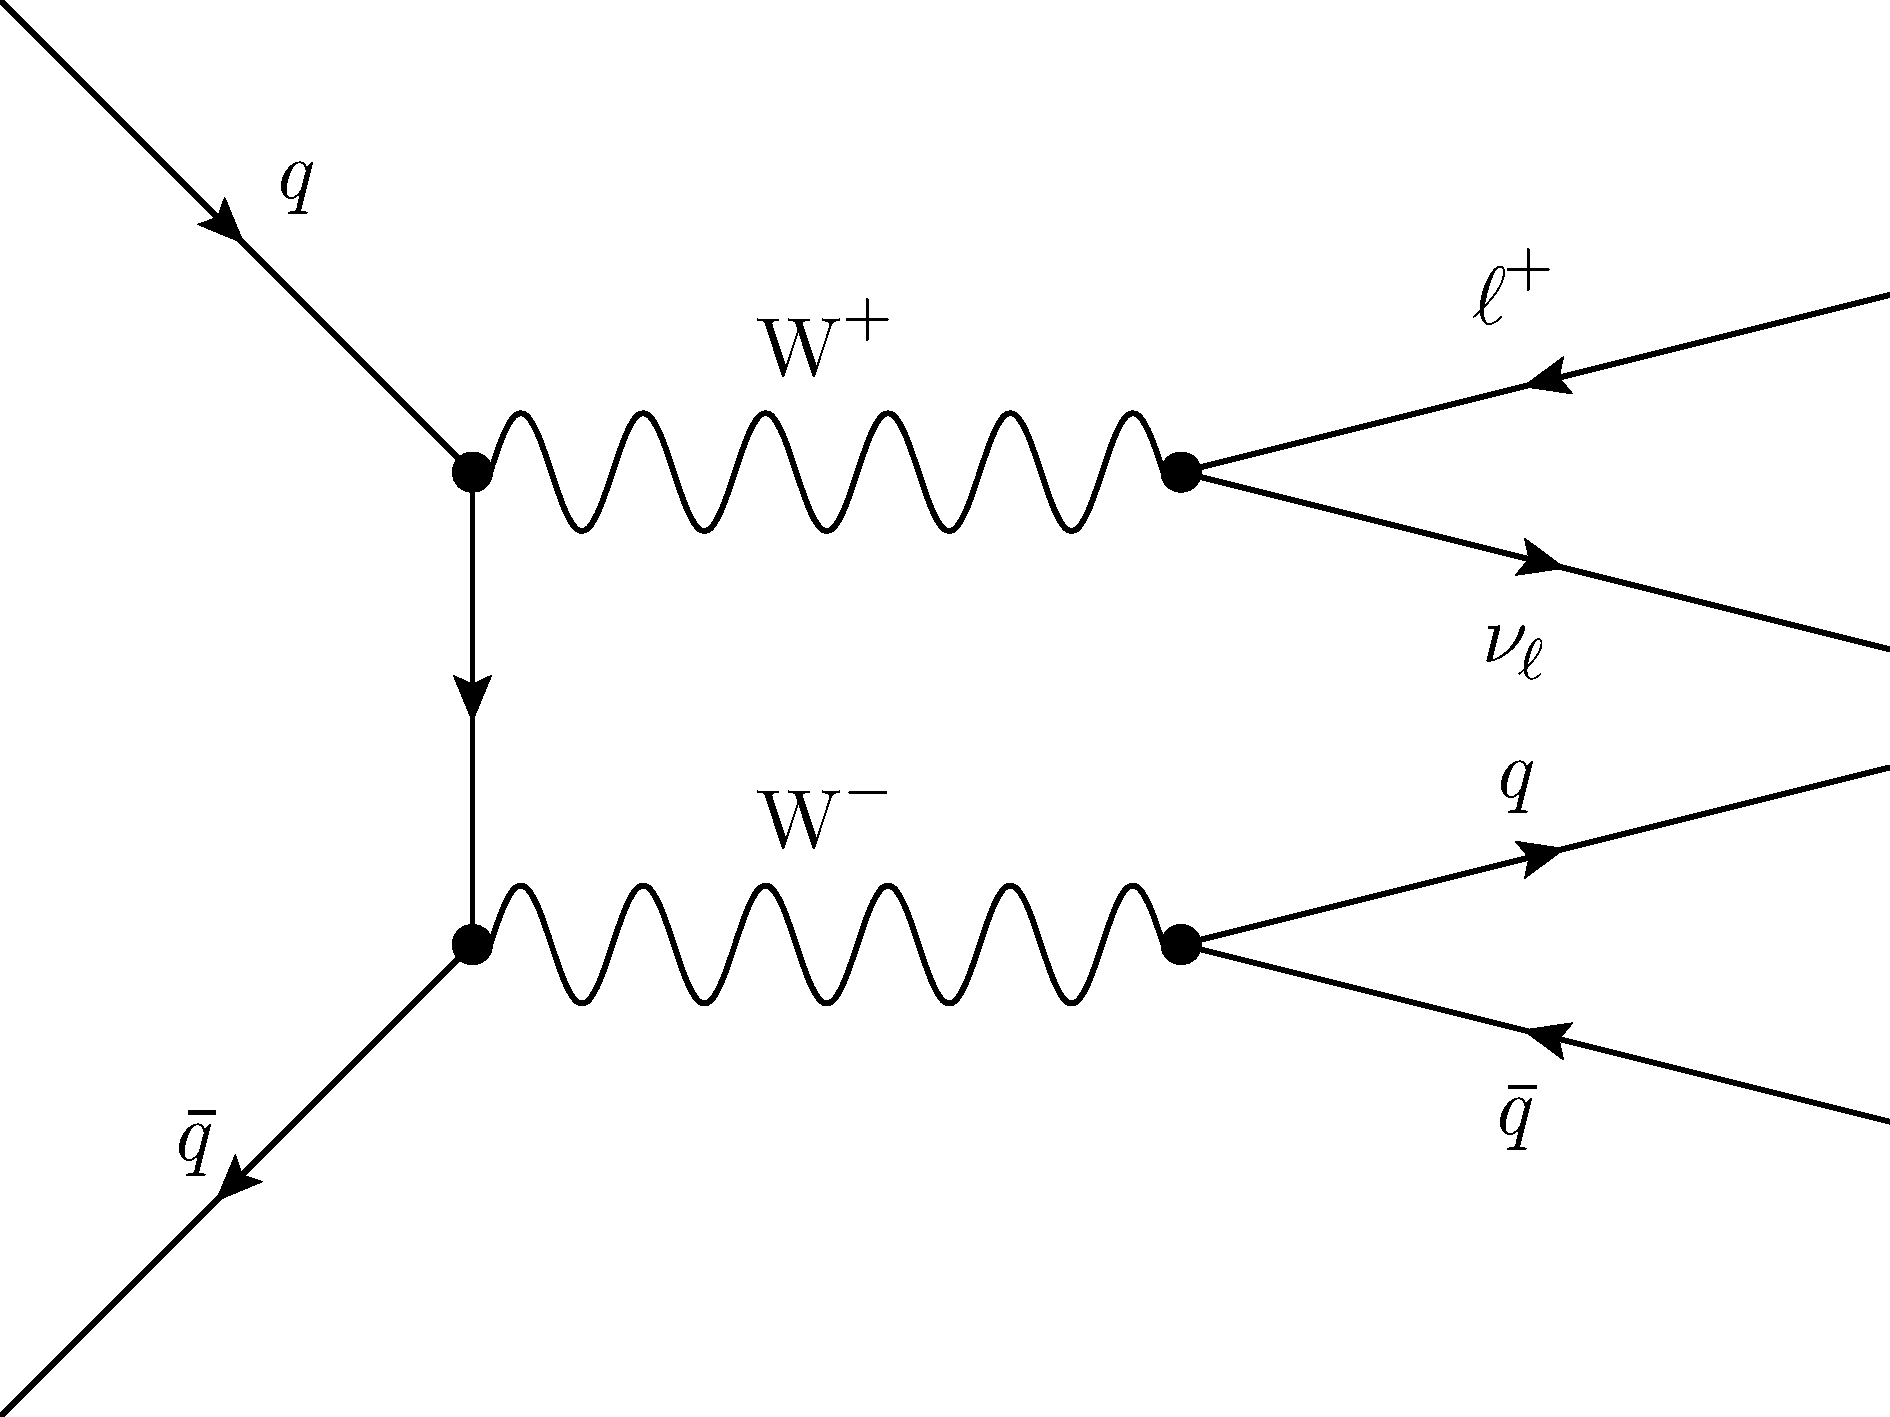
\includegraphics[width=\figwidth]{FeynmanDiagrams/WW.pdf}
      \caption{WW}
      \label{fig:WW}
    \end{subfigure}%
    ~ %add desired spacing between images, e. g. ~, \quad, \qquad etc. 
    %(or a blank line to force the subfigure onto a new line)
    \begin{subfigure}[b]{\figwidththree}
      \centering
      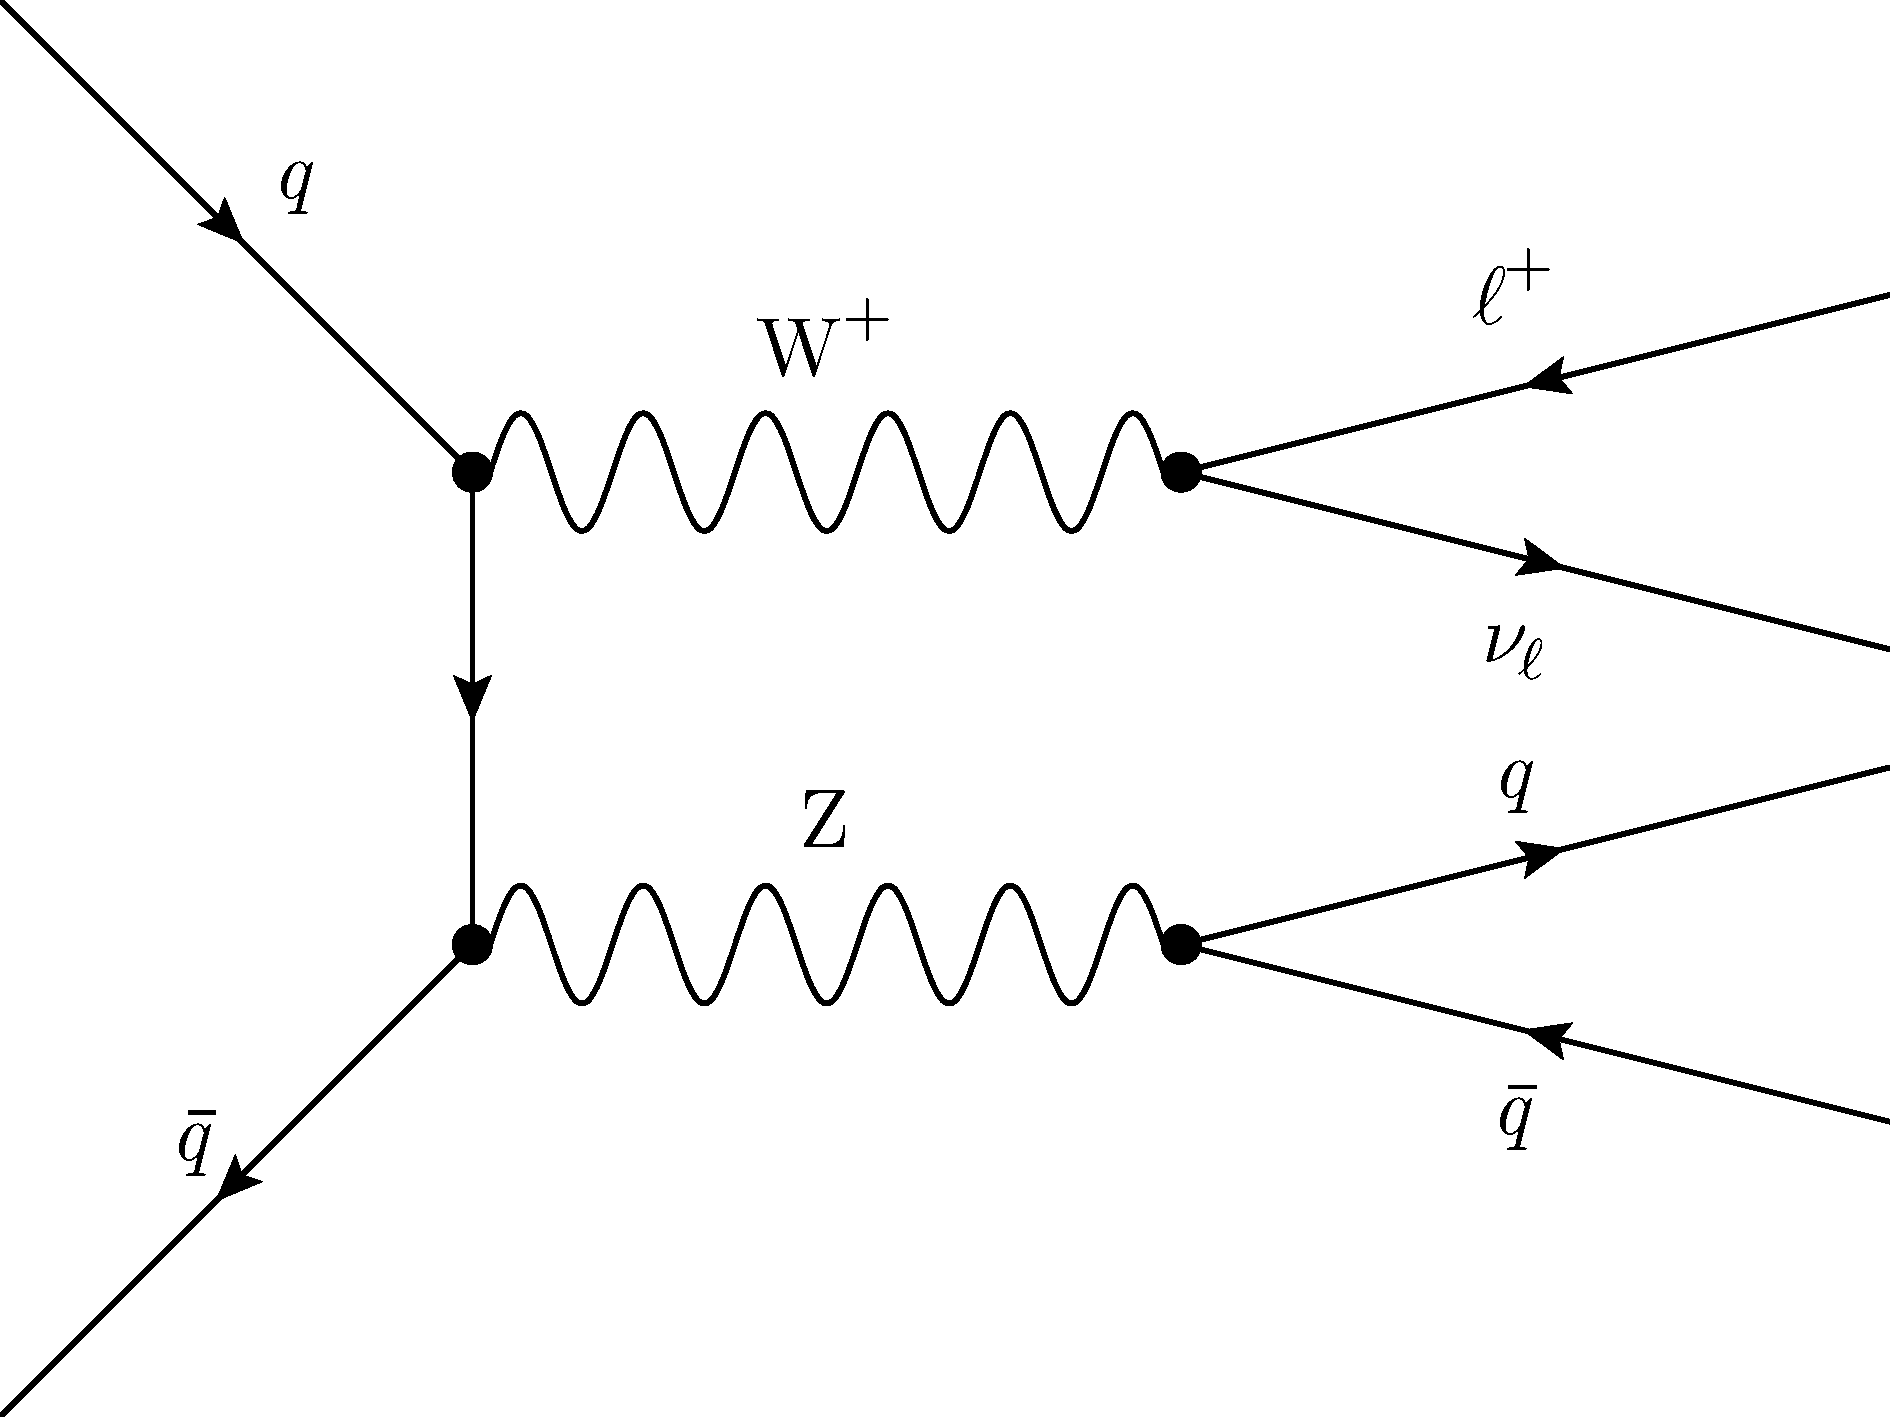
\includegraphics[width=\figwidth]{FeynmanDiagrams/WZ.pdf}
      \caption{WZ}
      \label{fig:WZ}
    \end{subfigure}
    ~
    \begin{subfigure}[b]{\figwidththree}
      \centering
      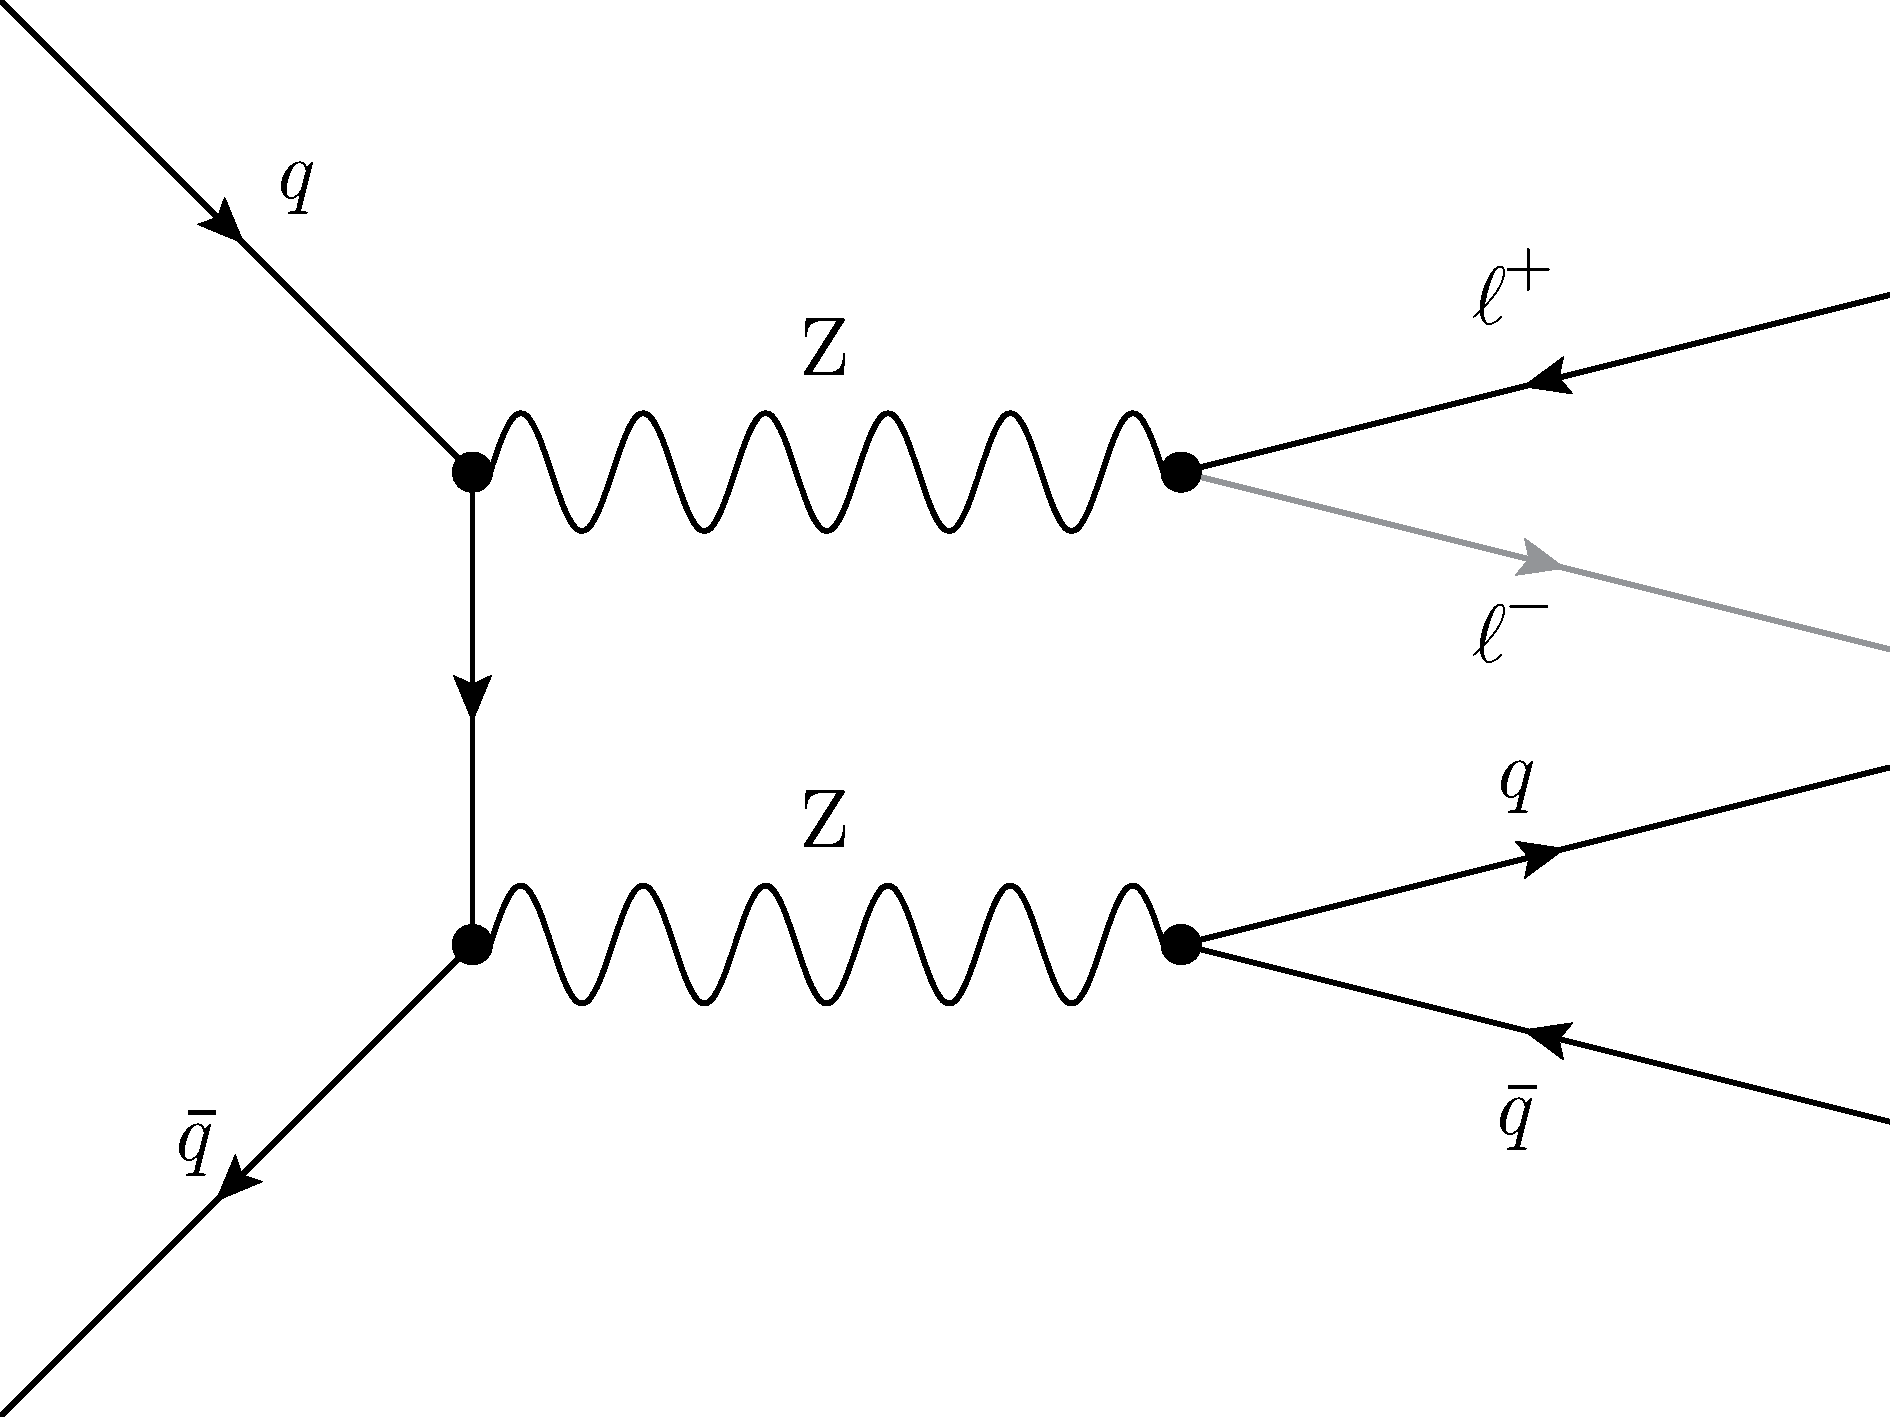
\includegraphics[width=\figwidth]{FeynmanDiagrams/ZZ.pdf}
      \caption{ZZ}
      \label{fig:ZZ}
    \end{subfigure}
    %\caption{Pictures of animals}\label{fig:STop}
  \end{figure}
}
\frame{
  \frametitle{Backgrounds}
  \framesubtitle{WJets}
  \vspace*{-0.24cm}
  \begin{block}{WJets}
    \scriptsize{
    \begin{itemize}
      \myitem Biggest background (82-88\% of background events)
      \myitem Same final state signature as our signal
      \myitem SM Cross-Section: $31314\pm1558\unit{pb}$
    \end{itemize}
    }
  \end{block}
  \begin{figure}
    \centering
    \begin{subfigure}[b]{\figwidththree}
      \centering
      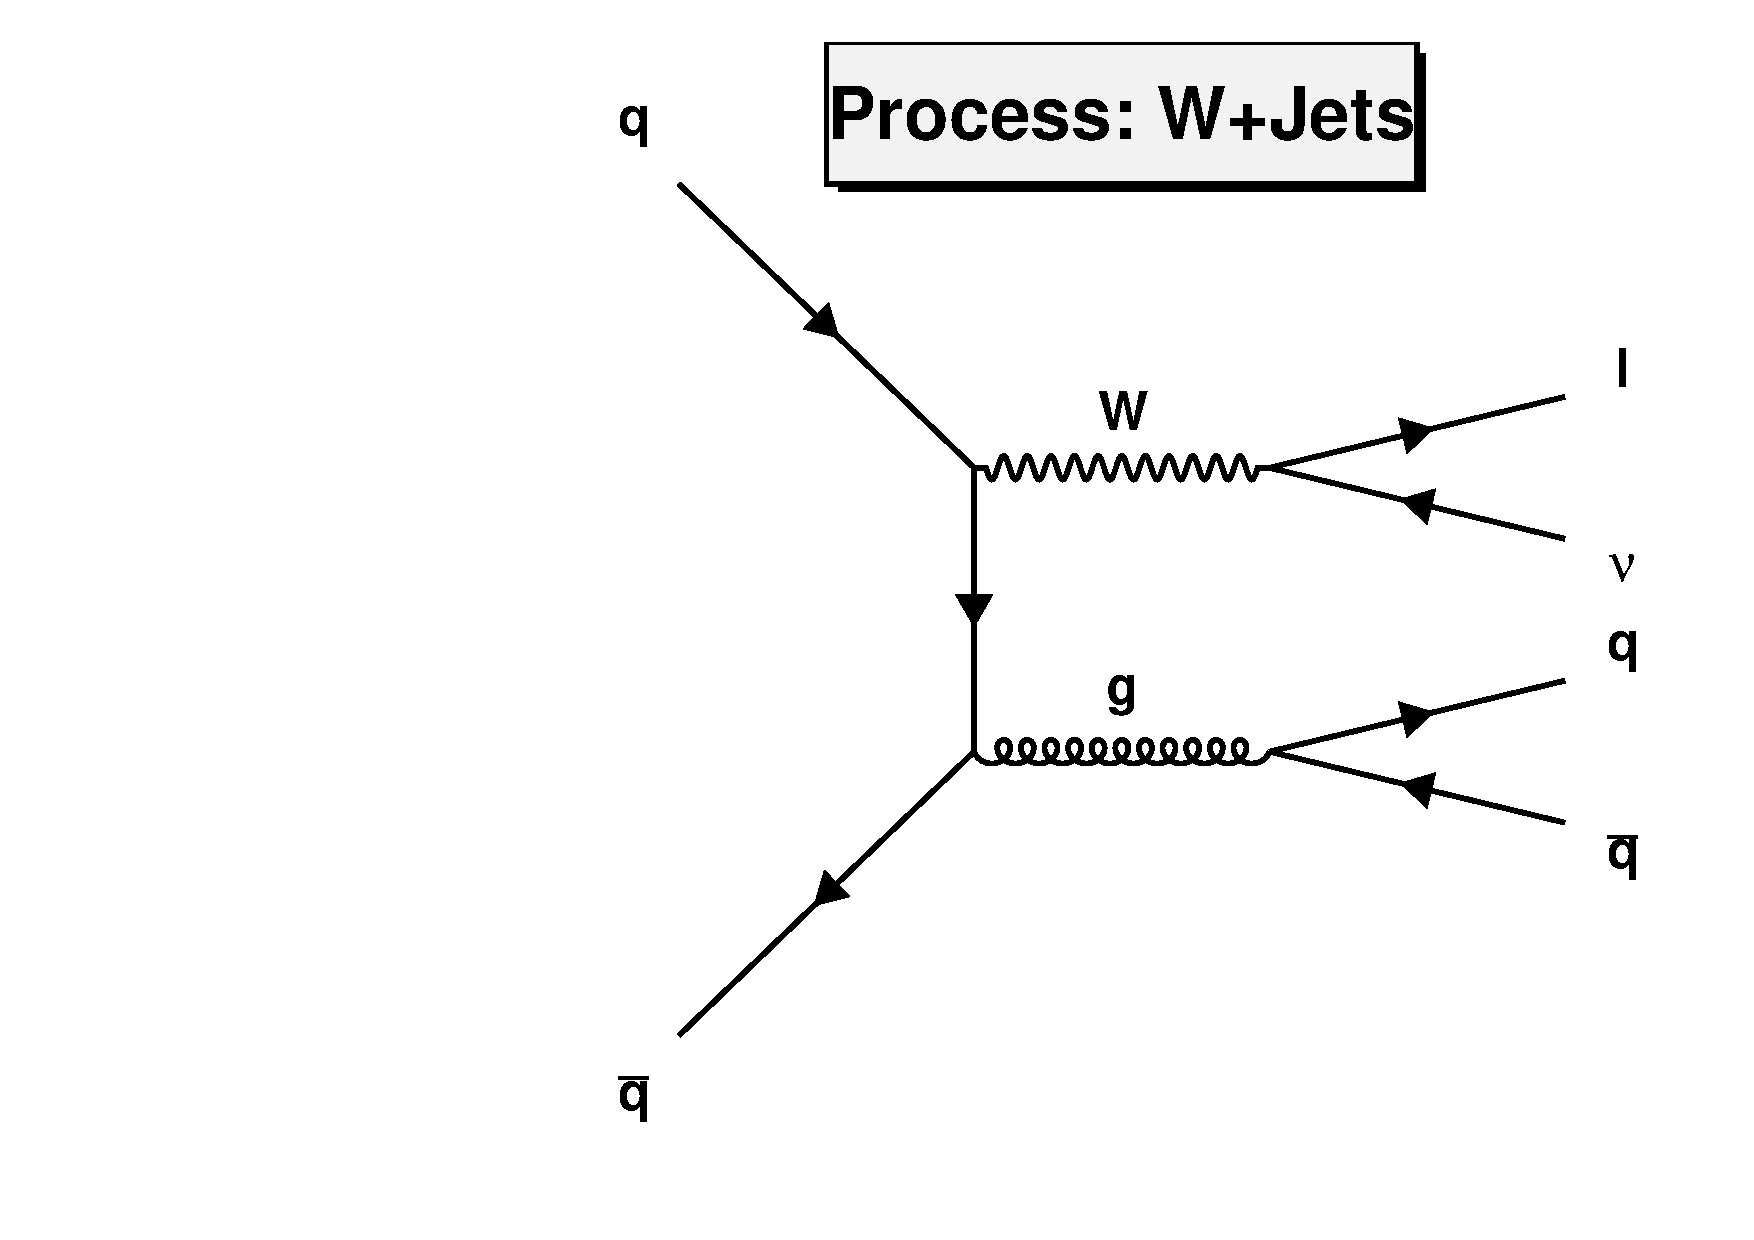
\includegraphics[width=\figwidth]{FeynmanDiagrams/WJets1.pdf}
      \caption{WJets1}
      \label{fig:WJets1}
    \end{subfigure}%
    ~ %add desired spacing between images, e. g. ~, \quad, \qquad etc. 
    %(or a blank line to force the subfigure onto a new line)
    \begin{subfigure}[b]{\figwidththree}
      \centering
      \includegraphics[width=\figwidth]{FeynmanDiagrams/WJets2.pdf}
      \caption{Wjets2}
      \label{fig:WJets2}
    \end{subfigure}
    ~ %add desired spacing between images, e. g. ~, \quad, \qquad etc. 
    %(or a blank line to force the subfigure onto a new line)
    \begin{subfigure}[b]{\figwidththree}
      \centering
      \includegraphics[width=\figwidth]{FeynmanDiagrams/WJets3.pdf}
      \caption{WJets3}
      \label{fig:WJets3}
    \end{subfigure}
    %\caption{Pictures of animals}\label{fig:STop}
  \end{figure}
}
\frame{
  \frametitle{Backgrounds continued...}
  \framesubtitle{ZJets, TTbar, and QCD}
  \vspace*{-0.51cm}
  \begin{columns}[T]
    \column{4.4cm}
    \begin{block}{ZJets}
      \scriptsize{
        \begin{itemize}
          \myitem Must miss a lepton to look like our signal
          \myitem SM Cross-Section: $3048\pm132\unit{pb}$
        \end{itemize}
      }
    \end{block}
    \column{7.4cm}
    \begin{block}{TTbar}
      \scriptsize{
        \begin{itemize}
          \myitem Must miss two jets to look like our signal
          \myitem Very reducible background (ex: using b-tagging, nJets,
          etc.)
          \myitem SM Cross-Section: $157.5\pm24.4\unit{pb}$
        \end{itemize}
      }
    \end{block}
  \end{columns}
  \vspace*{-0.15cm}
  \begin{block}{QCD}
    \scriptsize{
      \begin{itemize}
        \myitem Major background for the electron channel
        (smaller component in the muon channel)
        \myitem Hard to model (no precise cross-section)
        \myitem MC events created using a data driven method
      \end{itemize}
    }
  \end{block}
  \vspace*{-0.20cm}
  \begin{figure}
    \centering
    \begin{subfigure}[b]{0.29\textwidth}
      \centering
      \includegraphics[width=\figwidth]{FeynmanDiagrams/DYJets.pdf}
      \caption{ZJets}
      \label{fig:ZJets}
    \end{subfigure}%
    ~ %add desired spacing between images, e. g. ~, \quad, \qquad etc. 
    %(or a blank line to force the subfigure onto a new line)
    \begin{subfigure}[b]{0.29\textwidth}
      \centering
      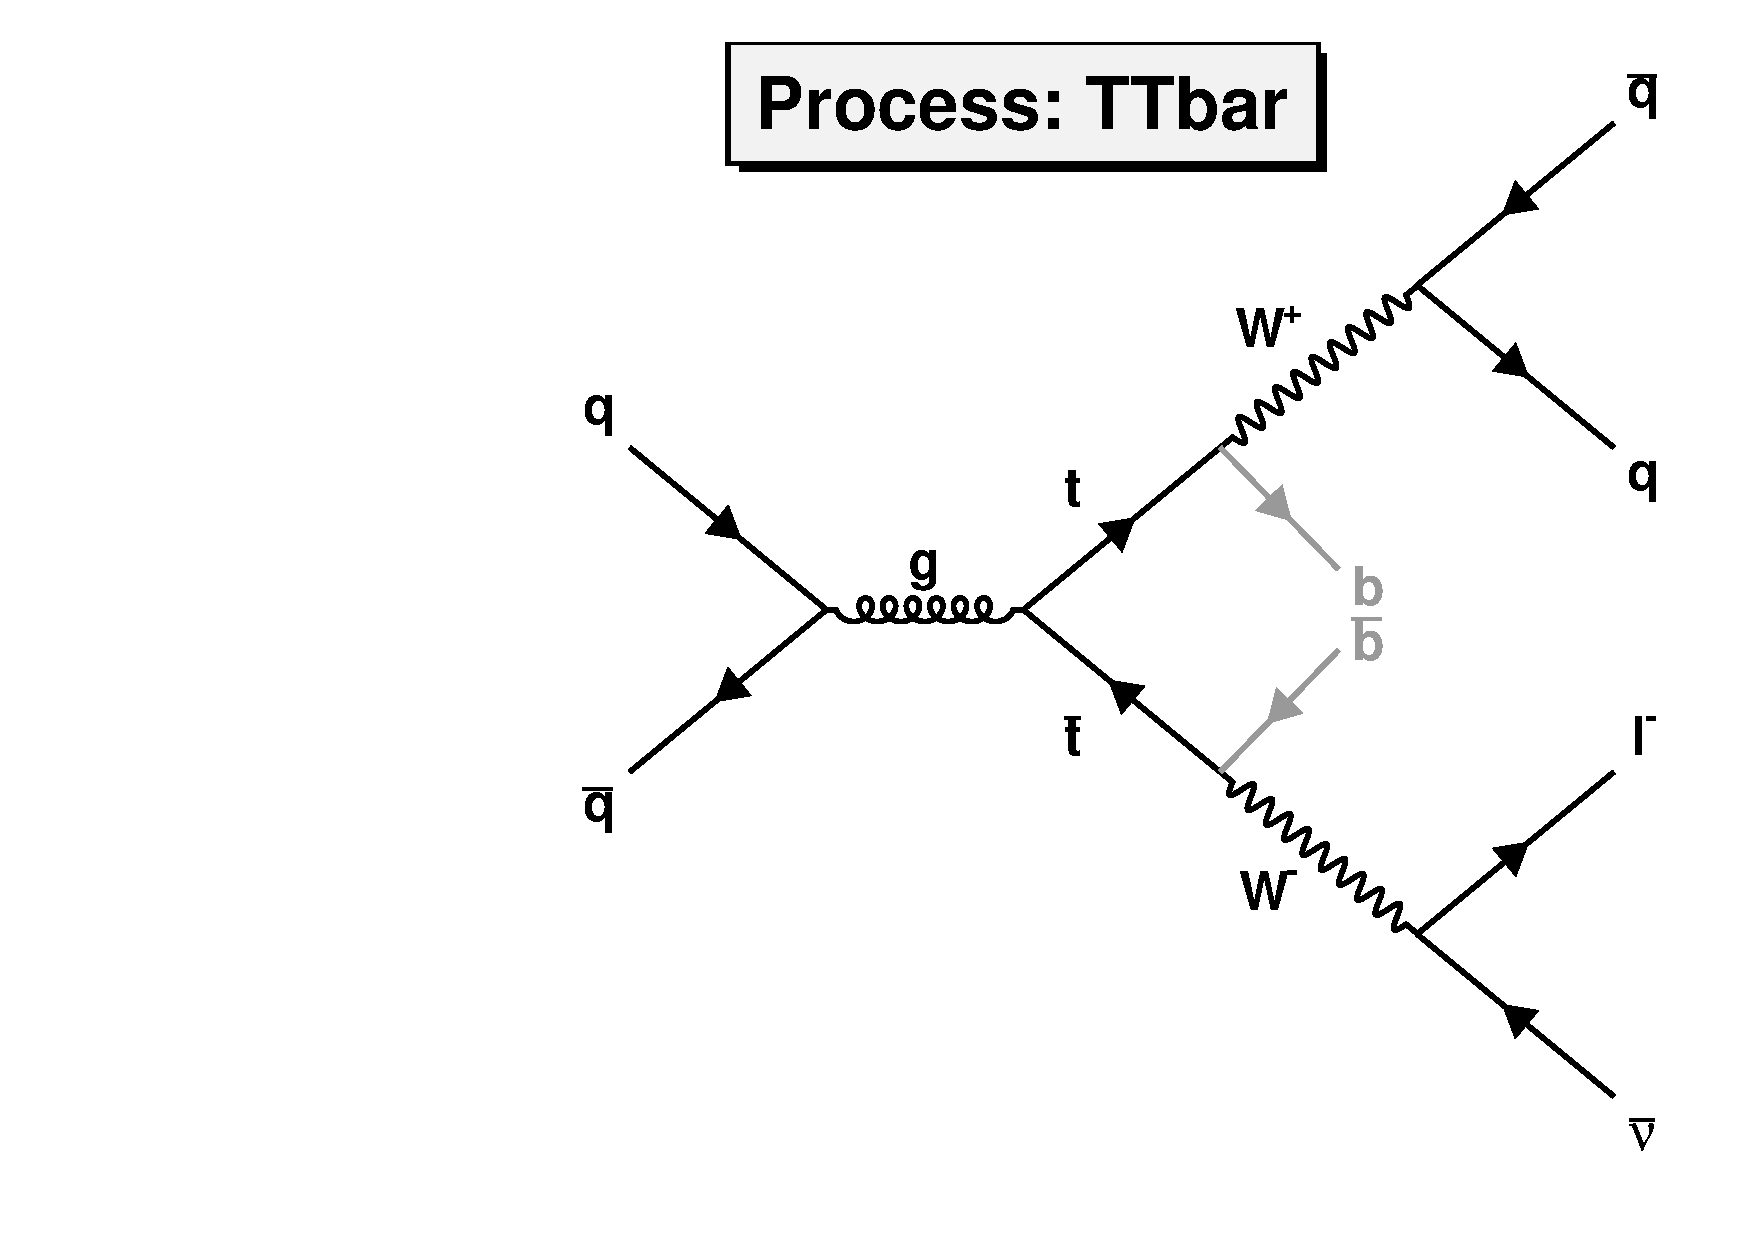
\includegraphics[width=\figwidth]{FeynmanDiagrams/TTbar.pdf}
      \caption{TTbar}
      \label{fig:TTbar}
    \end{subfigure}
    ~ %add desired spacing between images, e. g. ~, \quad, \qquad etc. 
    %(or a blank line to force the subfigure onto a new line)
    \begin{subfigure}[b]{0.29\textwidth}
      \centering
      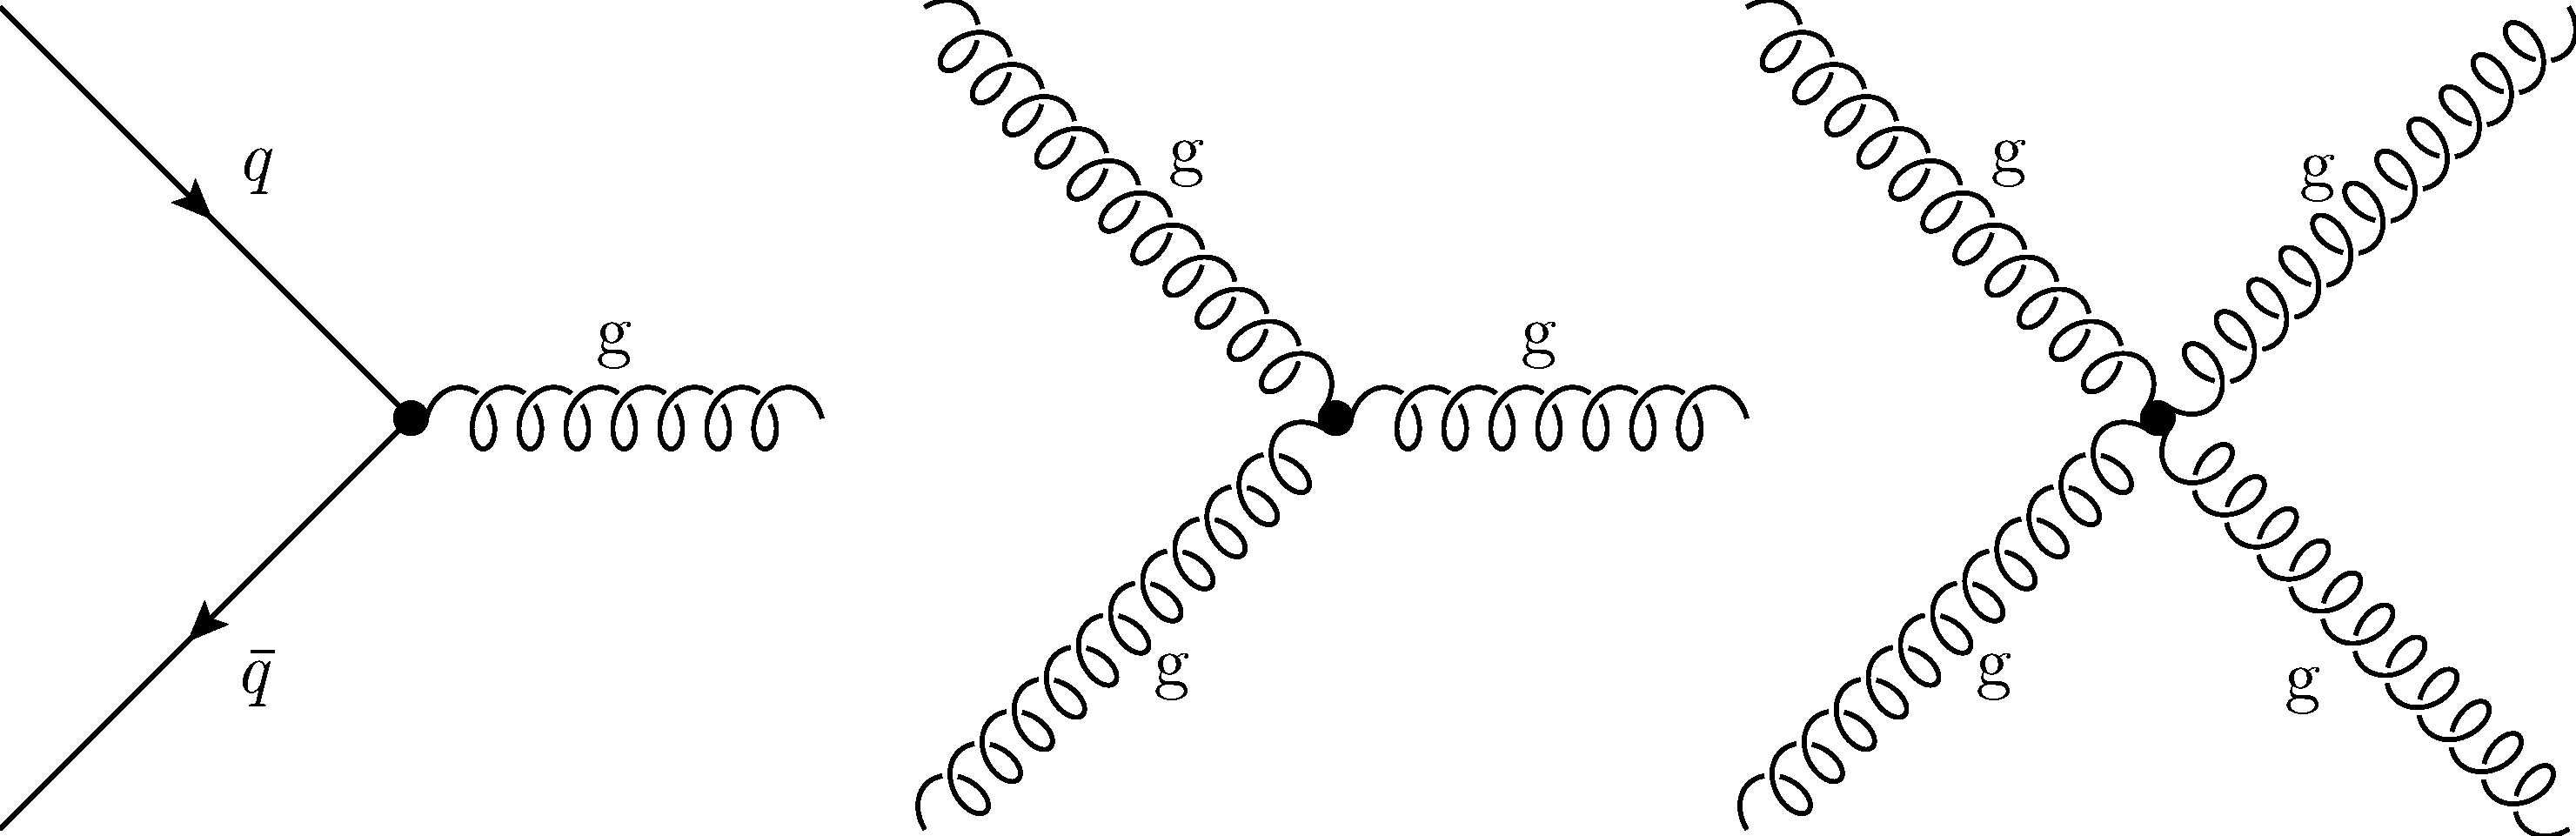
\includegraphics[width=\figwidth]{FeynmanDiagrams/QCD.pdf}
      \caption{QCD}
      \label{fig:QCD}
    \end{subfigure}
    %\caption{Pictures of animals}\label{fig:STop}
  \end{figure}
}
\frame{
  \frametitle{Backgrounds continued...}
  \framesubtitle{STopS, STopT, and STopTW}
  \vspace*{-0.24cm}
  \begin{block}{STop}
    \scriptsize{
    \begin{itemize}
      \myitem Small background
      \myitem Same final state as signal (except for TW channel)
      \myitem SM Cross-Sections:
      \begin{itemize}
        \scriptsize{
          \myitemtwo STopS\_T: $3.190\pm0.19\unit{pb}$
          \myitemtwo STopS\_Tbar: $1.440\pm0.08\unit{pb}$ 
          \myitemtwo STopT\_T: $41.92\pm2.42\unit{pb}$
          \myitemtwo STopT\_Tbar: $22.65\pm1.41\unit{pb}$ 
          \myitemtwo STopTW\_T: $7.870\pm0.77\unit{pb}$
          \myitemtwo STopTW\_Tbar: $7.870\pm0.77\unit{pb}$
        }
      \end{itemize}
    \end{itemize}
    }
  \end{block}
  \vspace*{-0.20cm}
  \begin{figure}
    \centering
    \begin{subfigure}[b]{\figwidththree}
      \centering
      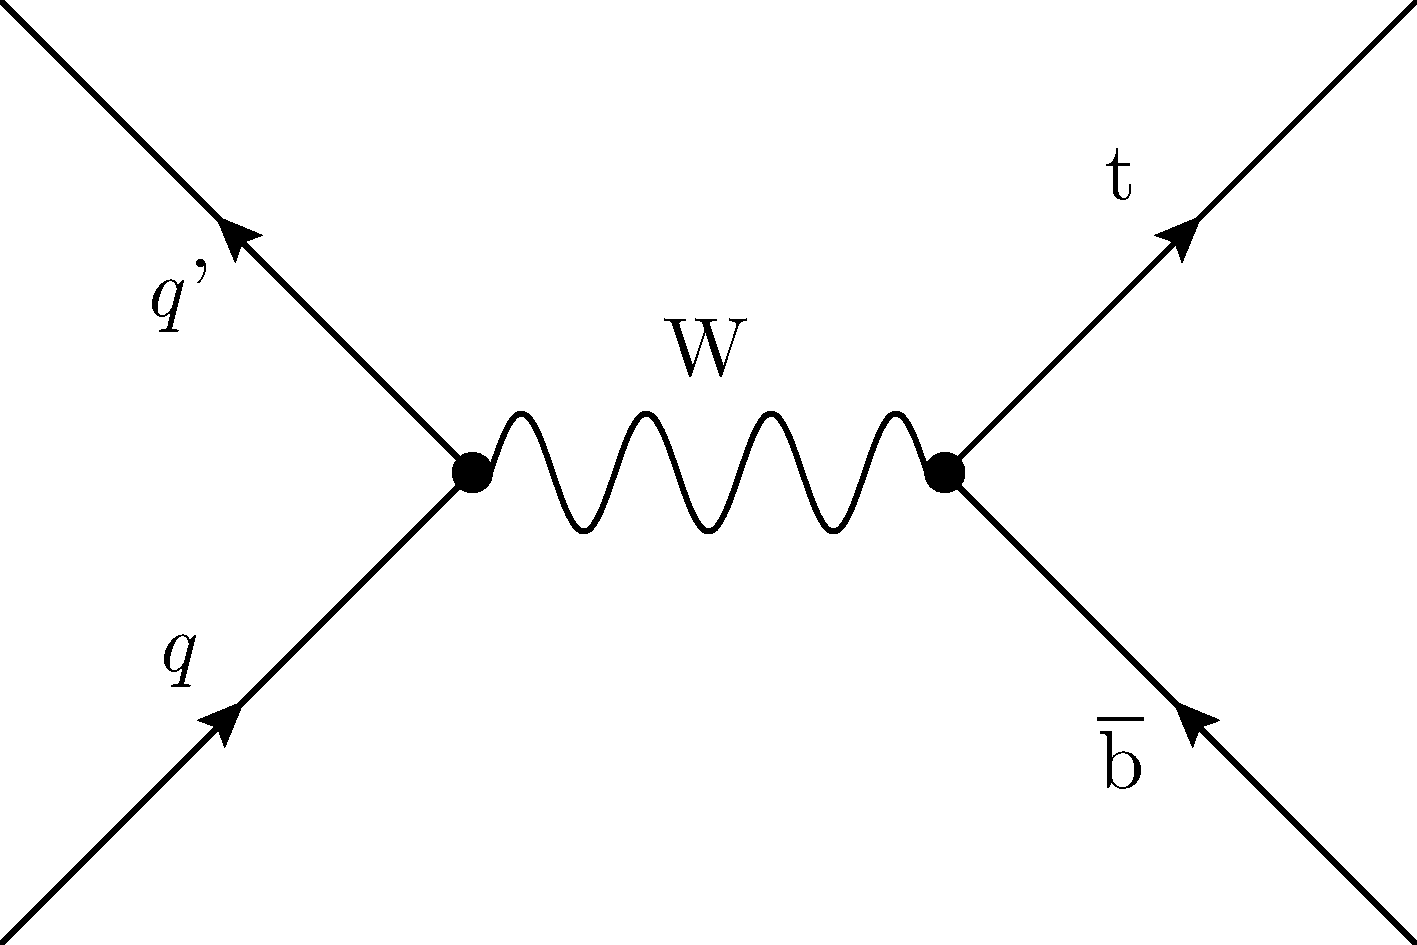
\includegraphics[width=\figwidth]{FeynmanDiagrams/STopS.pdf}
      \caption{STopS}
      \label{fig:STopS}
    \end{subfigure}%
    ~ %add desired spacing between images, e. g. ~, \quad, \qquad etc. 
    %(or a blank line to force the subfigure onto a new line)
    \begin{subfigure}[b]{\figwidththree}
      \centering
      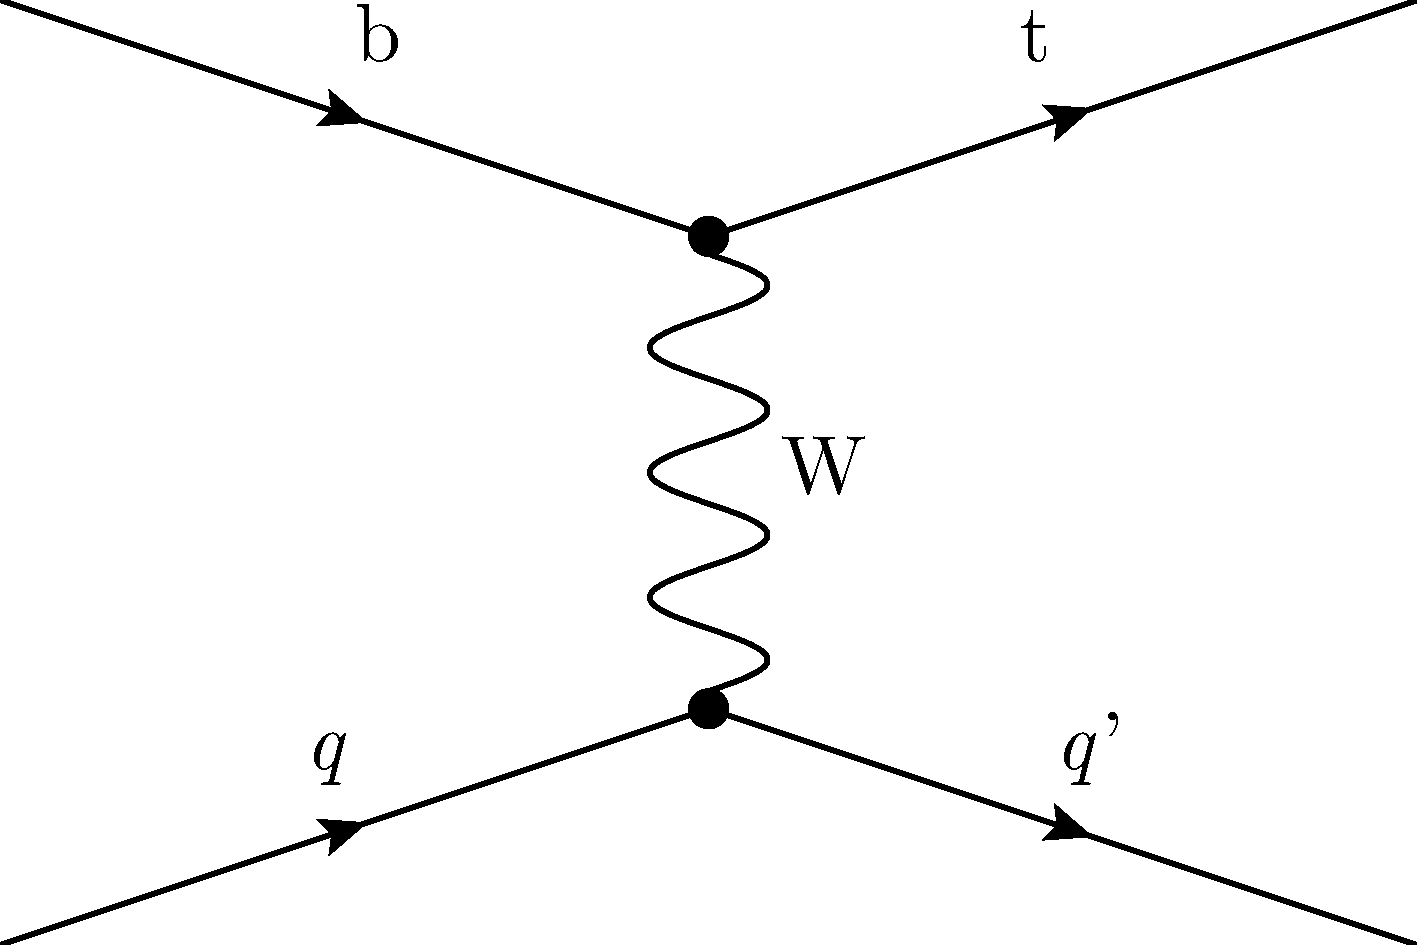
\includegraphics[width=\figwidth]{FeynmanDiagrams/STopT.pdf}
      \caption{STopT}
      \label{fig:STopT}
    \end{subfigure}
    ~ %add desired spacing between images, e. g. ~, \quad, \qquad etc. 
    %(or a blank line to force the subfigure onto a new line)
    \begin{subfigure}[b]{\figwidththree}
      \centering
      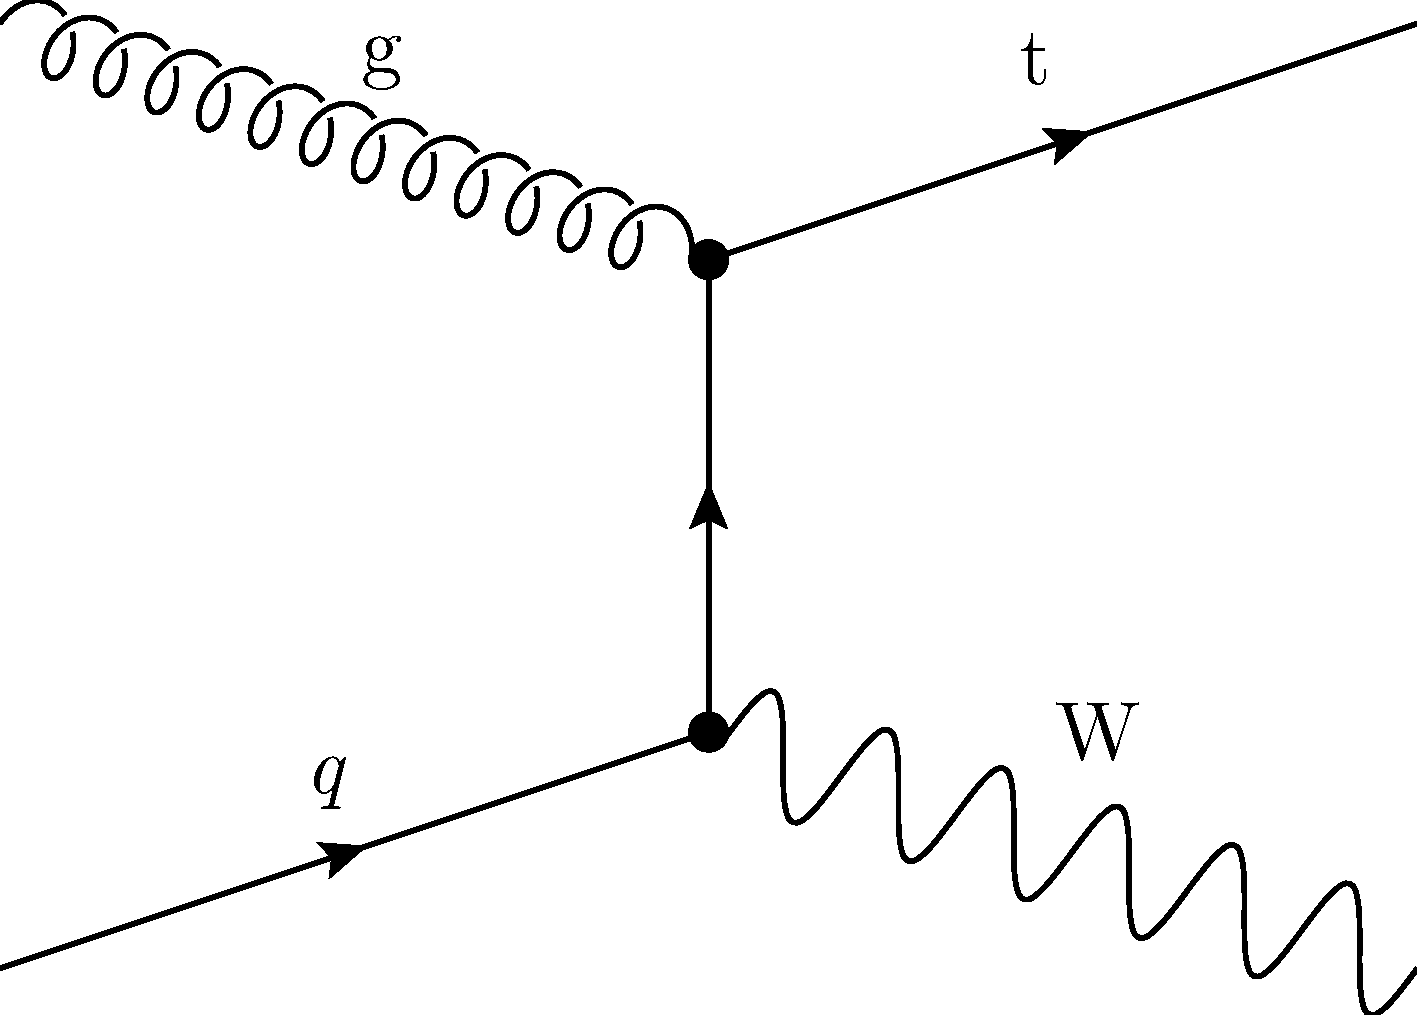
\includegraphics[width=\figwidth]{FeynmanDiagrams/STopTW.pdf}
      \caption{STopTW}
      \label{fig:STopTW}
    \end{subfigure}
    %\caption{Pictures of animals}\label{fig:STop}
  \end{figure}
}

\subsection{Event Selection}
\frame{
  \frametitle{Event Selection}
  \vspace*{-0.24cm}
  \begin{block}{Baseline Selection}
    \begin{columns}[T]
      \column{5cm}
      \begin{enumerate}
        \tiny{
          \item Trigger
          \begin{itemize}
            \tiny{
              \myitemtwo Single Muon (Electron) Triggers
            }
          \end{itemize}
          \item 1 good PV
          \item $>=1$ ``tight'' lepton
          \item 1 ``tight'' lepton, 0 ``loose'' leptons
          \begin{itemize}
            \tiny{
              \myitemtwo 1 tight muon, 0 tight electrons
              \myitemtwo 1 tight electron, 0 tight muons
            }
          \end{itemize}
          \item $>=2$ jets
          \item $\met>25\unit{GeV}$
        }
      \end{enumerate}
      \column{6cm}
      \begin{itemize}
        \scriptsize{
          \myitem tight - Refers to a set of selection criteria for an
          object which make sure that the object is well defined, but
          may also have a lower selection efficiency
          \myitem loose - Another set of selection criteria, for the
          same object, but the cuts are more inclusive. This set of
          criteria have a higher selection efficiency, but also a higher
          rate of misidentification
        }
      \end{itemize}
    \end{columns}
  \end{block}
  \vspace*{-0.49cm}
  \begin{columns}[T]
    \column{5.8cm}
    \begin{block}{Muons}
      \begin{itemize}
        \tiny{
          \myitem $p_{T}^{muon}>20\unit{GeV}$
          \myitem $|\eta^{muon}|<2.1$
          \myitem etc.
        }
      \end{itemize}
    \end{block}
    \column{5.8cm}
    \begin{block}{Electrons}
      \begin{itemize}
        \tiny{
          \myitem $p_{T}^{electron}>20\unit{GeV}$
          \myitem $|\eta^{electron}|<2.5$
          \myitem etc.
        }
      \end{itemize}
    \end{block}
  \end{columns}
  \vspace*{-0.15cm}
  \begin{block}{Jets}
    \begin{itemize}
      \tiny{
        \myitem Anti-kT ($R=0.5$) Particle Flow Jets
        \myitem Full jet energy correction (JEC) factorized approach
        implemented, including charged hadron subtraction (CHS) for
        pileup removal
        \myitem $p_{T}^{jet}>20\unit{GeV}$ (removes low $p_{T}$ jets)
        \myitem $|\eta^{jet}|<2.4$ (keeps jets in tracker region)
        \myitem ${\Delta}R(lepton,jet)>0.3$ (for good isolation)
      }
    \end{itemize}
  \end{block}
}
\frame{
  \frametitle{Analysis Level Selection}
  \vspace*{-0.24cm}
  \begin{block}{Diboson Analysis Cuts}
    \scriptsize{
      \begin{itemize}
        \myitem Muon (electron) $p_{T}>25(35)\unit{GeV}$
        \myitem $\met>25(30)\unit{GeV}$ for muon (electron) samples
        \myitem $p_{T}^{jet}>35\unit{GeV}$
        \myitem $|{\Delta}{\eta}_{jj}|<1.5$
        \myitem Dijet $p_{T}>20\unit{GeV}$
        \myitem $|{\Delta}{\phi}(\met,leadjet)|>0.4$
        \myitem W transverse mass $>50\unit{GeV}$
      \end{itemize}
    }
  \end{block}
  \begin{table}[h]\normalsize
    \begin{tabular}{|c|c|c|}
      \hline
      \textbf{Process Muon(Electron)} & \textbf{Baseline Cuts}  & \textbf{Analysis Level Cuts}\\
                                      & \textbf{Yield (\# evts)} & \textbf{Yield (\# evts)}\\
      \hline
      Diboson & 8136.66 (6151.72) & 699.922 (391.202)\\
      WJets   & 813555 (333646)   & 37796.5 (18498.3)\\
      ZJets   & 65116.6 (47876.4) & 1619.66 (773.659)\\
      TTbar   & 7862.26 (5991.55) & 1385.82 (868.484)\\
      STop    & 9482.4 (7071.11)  & 985.688 (526.434)\\
      QCD     & 165287 (261826)   & 104.813 (1395)\\
      \hline
      Sum     & 1069440 (662563)  & 42592.4 (22453)\\
      \hline
      Data    & 1013270 (538166)  & 42391 (22210)\\
      \hline
   \end{tabular}
    \label{tab:AnaCutFlow}
  \end{table}
}
\frame{
  \frametitle{Validation Plots}
  \framesubtitle{Lepton $p_{T}$ Cut}
  \vspace*{-0.54cm}
  \begin{columns}[T]
    \column{5.5cm}
    \begin{block}{Baseline Cuts}
      \begin{center}
        \includegraphics[width=\figwidthminus]{ValidationPlotsNoCuts/LeptPt_electron.pdf}\\
        \includegraphics[width=\figwidthminus]{ValidationPlotsNoCuts/LeptPt_muon.pdf}
      \end{center}
    \end{block}
    \column{5.5cm}
    \begin{block}{Analysis Level Cuts}
      \begin{center}
        \includegraphics[width=\figwidthminus]{ValidationPlots/LeptPt_electron.pdf}\\
        \includegraphics[width=\figwidthminus]{ValidationPlots/LeptPt_muon.pdf}
      \end{center}
    \end{block}
  \end{columns}
}
\frame{
  \frametitle{Validation Plots}
  \framesubtitle{$\met$ Cut}
  \vspace*{-0.54cm}
  \begin{columns}[T]
    \column{5.5cm}
    \begin{block}{Baseline Cuts}
      \begin{center}
        \includegraphics[width=\figwidthminus]{ValidationPlotsNoCuts/MET_electron.pdf}\\
        \includegraphics[width=\figwidthminus]{ValidationPlotsNoCuts/MET_muon.pdf}
      \end{center}
    \end{block}
    \column{5.5cm}
    \begin{block}{Analysis Level Cuts}
      \begin{center}
        \includegraphics[width=\figwidthminus]{ValidationPlots/MET_electron.pdf}\\
        \includegraphics[width=\figwidthminus]{ValidationPlots/MET_muon.pdf}
      \end{center}
    \end{block}
  \end{columns}
}
\frame{
  \frametitle{Validation Plots}
  \framesubtitle{$p_{T}^{Jet1}$ and $p_{T}^{Jet2}$}
  \vspace*{-0.54cm}
  \begin{columns}[T]
    \column{5.5cm}
    \begin{block}{$p_{T}^{Jet1}$}
      \begin{center}
        \includegraphics[width=\figwidthminus]{ValidationPlots/Jet1Pt_electron.pdf}\\
        \includegraphics[width=\figwidthminus]{ValidationPlots/Jet1Pt_muon.pdf}
      \end{center}
    \end{block}
    \column{5.5cm}
    \begin{block}{$p_{T}^{Jet2}$}
      \begin{center}
        \includegraphics[width=\figwidthminus]{ValidationPlots/Jet2Pt_electron.pdf}\\
        \includegraphics[width=\figwidthminus]{ValidationPlots/Jet2Pt_muon.pdf}
      \end{center}
    \end{block}
  \end{columns}
}
\frame{
  \frametitle{Validation Plots}
  \framesubtitle{${\Delta}{\eta}_{jj}$ and Dijet $p_{T}$}
  \vspace*{-0.54cm}
  \begin{columns}[T]
    \column{5.5cm}
    \begin{block}{${\Delta}{\eta}_{jj}$}
      \begin{center}
        \includegraphics[width=\figwidthminus]{ValidationPlots/DeltaEtaJ1J2_electron.pdf}\\
        \includegraphics[width=\figwidthminus]{ValidationPlots/DeltaEtaJ1J2_muon.pdf}
      \end{center}
    \end{block}
    \column{5.5cm}
    \begin{block}{Dijet $p_{T}$}
      \begin{center}
        \includegraphics[width=\figwidthminus]{ValidationPlots/Ptjj_electron.pdf}\\
        \includegraphics[width=\figwidthminus]{ValidationPlots/Ptjj_muon.pdf}
      \end{center}
    \end{block}
  \end{columns}
}
\frame{
  \frametitle{Validation Plots}
  \framesubtitle{${\Delta}{\phi}(\met,leadjet)$ and W transverse mass}
  \vspace*{-0.54cm}
  \begin{columns}[T]
    \column{5.5cm}
    \begin{block}{${\Delta}{\phi}(\met,leadjet)$}
      \begin{center}
        \includegraphics[width=\figwidthminus]{ValidationPlots/DeltaPhi_METJ1_electron.pdf}\\
        \includegraphics[width=\figwidthminus]{ValidationPlots/DeltaPhi_METJ1_muon.pdf}
      \end{center}
    \end{block}
    \column{5.5cm}
    \begin{block}{W transverse mass}
      \begin{center}
        \includegraphics[width=\figwidthminus]{ValidationPlots/WmT_electron.pdf}\\
        \includegraphics[width=\figwidthminus]{ValidationPlots/WmT_muon.pdf}
      \end{center}
    \end{block}
  \end{columns}
}
\frame{
  \frametitle{Validation Plots}
  \framesubtitle{$M_{jj}$ and $M_{l{\nu}jj}$}
  \vspace*{-0.54cm}
  \begin{columns}[T]
    \column{5.5cm}
    \begin{block}{$M_{jj}$}
      \begin{center}
        \includegraphics[width=\figwidthminus]{ValidationPlots/Mjj_electron.pdf}\\
        \includegraphics[width=\figwidthminus]{ValidationPlots/Mjj_muon.pdf}
      \end{center}
    \end{block}
    \column{5.5cm}
    \begin{block}{$M_{l{\nu}jj}$}
      \begin{center}
        \includegraphics[width=\figwidthminus]{ValidationPlots/Mlvjj_electron.pdf}\\
        \includegraphics[width=\figwidthminus]{ValidationPlots/Mlvjj_muon.pdf}
      \end{center}
    \end{block}
  \end{columns}
}
\subsection{Matrix Element Technique}
\frame
{
  \begin{center}
    \begin{block}{}
      \begin{center}
        {\Huge{\textbf{How to Find the Diboson Cross Section}}}\\
        {\huge{\textbf{{\newline}Analysis Methodology}}}
      \end{center}
    \end{block}
  \end{center}
}
\subsubsection{A Little Bit Of Theory}
\frame{
  \frametitle{Types of Searches}
  \vspace*{-0.24cm}
  \begin{block}{Previous Generation of Searches}
    \scriptsize{
    \begin{itemize}
      \myitem Cut-and-count experiment
      \begin{itemize}
          \myitemtwo \scriptsize{Simplistic and not nearly sensitive enough for a Higgs search with high
          backgrounds}
      \end{itemize}
      \myitem Fit to a sensitive kinematic distribution
      \begin{itemize}
          \myitemtwo \scriptsize{More sensitive than event counting, but a fit to a single distribution excludes
          information from all other distributions}
        \end{itemize}
    \end{itemize}
    }
  \end{block}
  \vspace*{-0.15cm}
  \begin{block}{Matrix Element}
    \scriptsize{
      \begin{itemize}
        \myitem Uses the field theoretic differential cross section calculation to determine how
        likely an event is to come from a specific process.
      \end{itemize}
      \vspace*{-0.5cm}
      \begin{columns}[t]
        \column{5.5cm}
        \vspace*{-0.15cm}
        \begin{equation}\label{eq:dsigma1}
          d{\sigma}=|M|^{2}\frac{\hbar^{2}S}{4\sqrt{(q_{1}{\cdot}q_{2})^{2}-(m_{1}m_{2}c^{2})^{2}}}d{\Phi}_{n}
        \end{equation}
        \begin{equation}\label{eq:phasespace}
          d{\Phi}_{n}={\delta}(q_{1}+q_{2}-\sum_{i=1}^{n}p_{i})\prod_{i=1}^{n}\frac{cd^{3}p_{i}}{(2\pi)^{3}2E_{i}}
        \end{equation}
        \column{2.5cm}
        \vspace*{0.1cm}
        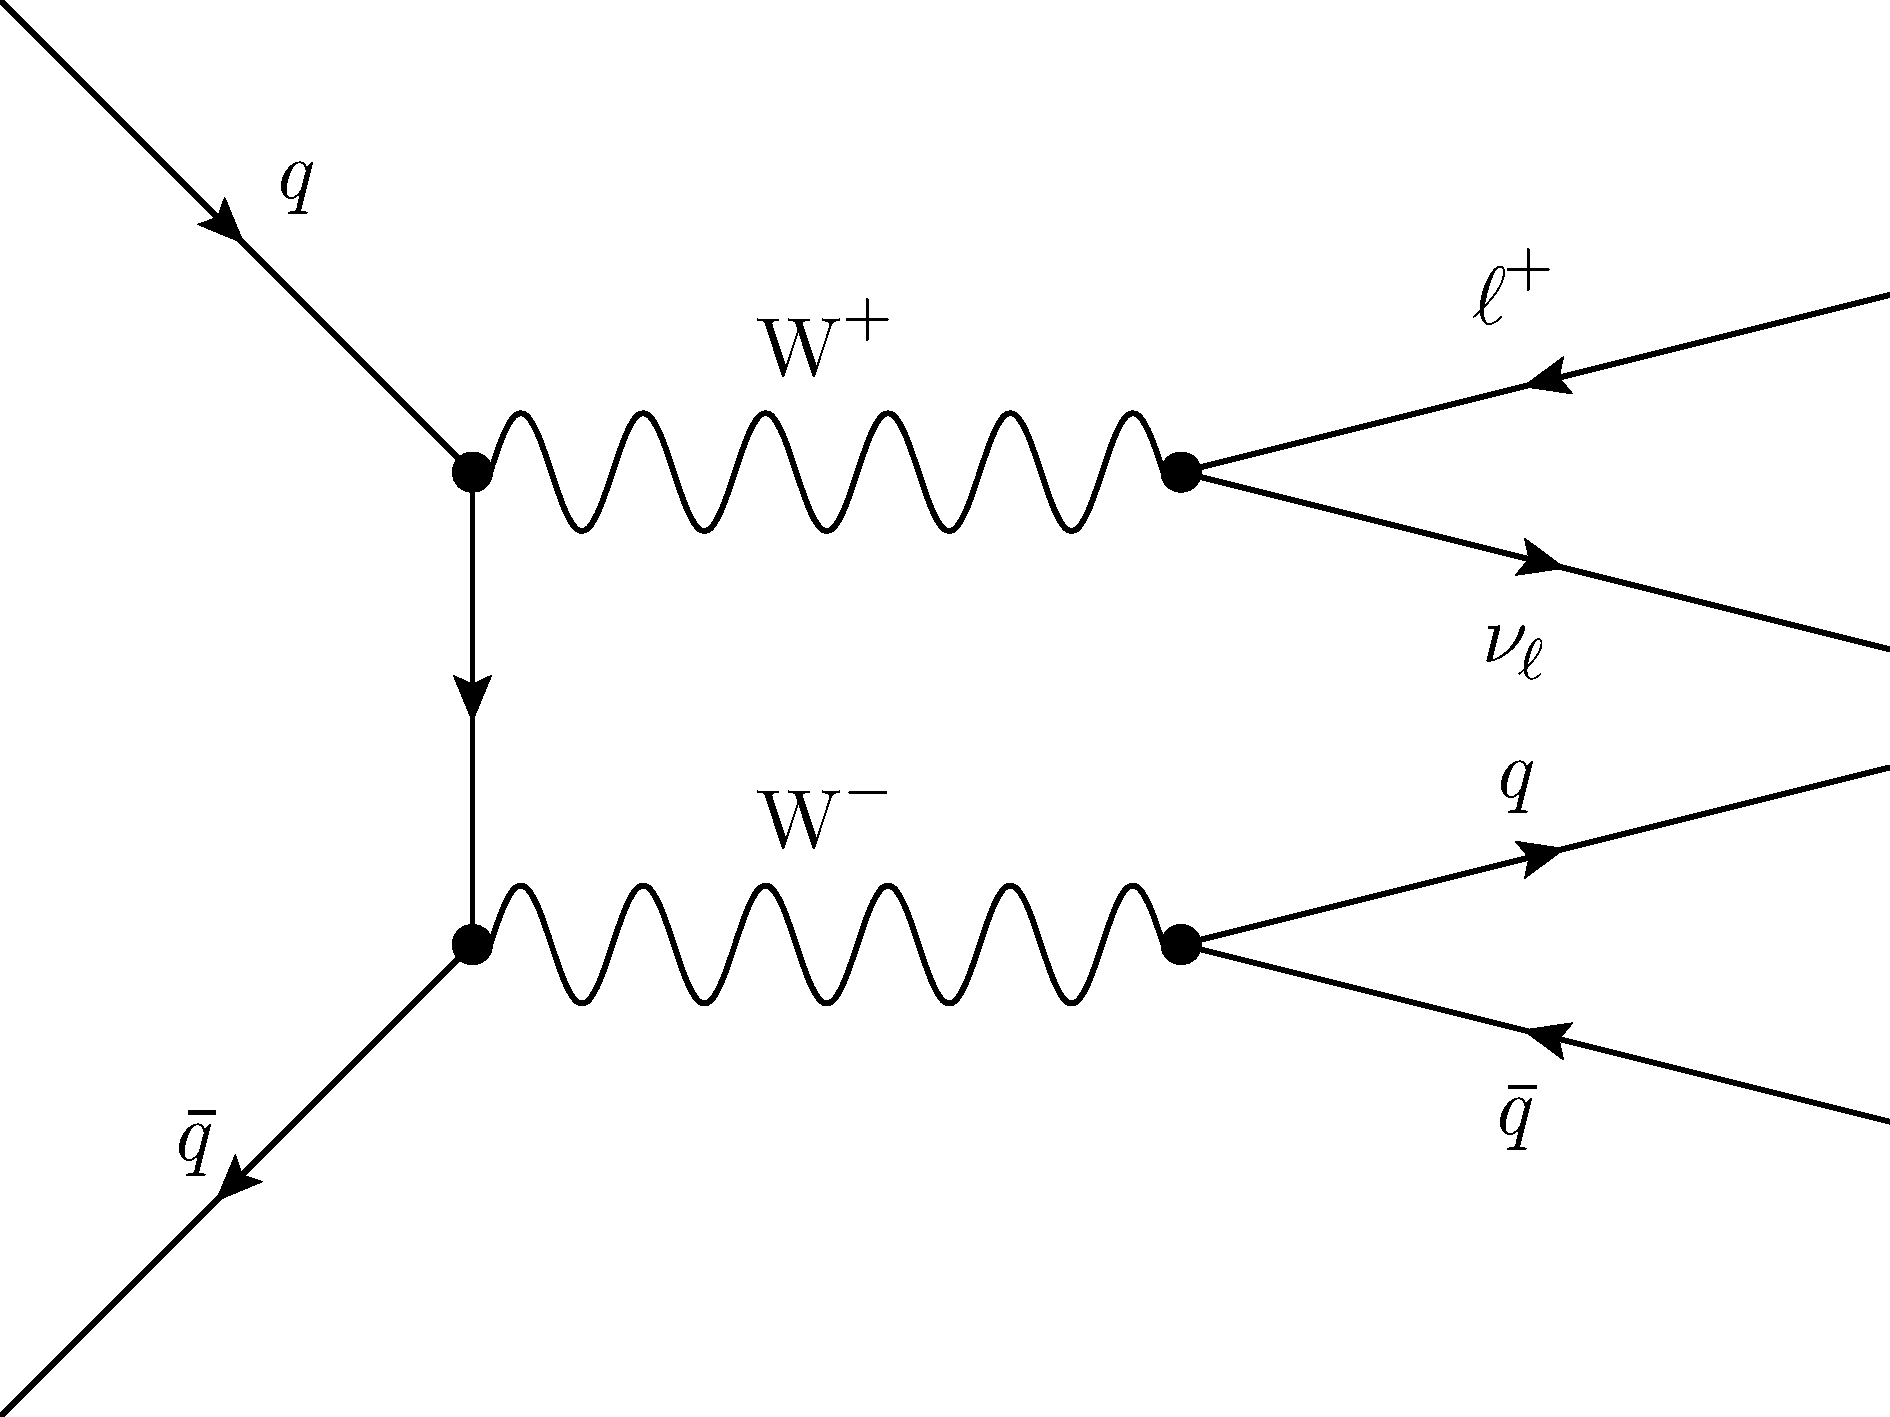
\includegraphics[width=\figwidth]{FeynmanDiagrams/WW.pdf}
      \end{columns}
      \begin{itemize}
        \myitem \eqref{eq:dsigma1} is the differential cross section and \eqref{eq:phasespace} is the phase space parameter
        \myitem M is the ME (amplitude) for the interaction and S is a combinatorial factor which takes
        into account identical particles.
        \myitem The phase space factor guarantees that each particle lies on its mass shell, the
        energy is positive, and that energy and momentum are conserved.
      \end{itemize}
    }
  \end{block}
}

\frame{
  \frametitle{Types of Searches}
  \vspace*{-0.24cm}
  \begin{block}{ME continued...}
    \scriptsize{
      \begin{itemize}
        \myitem With the introduction of parton distribution functions (PDFs), transfer functions, and
        constrains (see \eqref{eq:constraints} for sample), the differential cross section becomes:
      \end{itemize}
      \begin{equation}\label{eq:dsigma2}
        d{\sigma}={\int}dp_{z_{\nu}}|M|^{2}\frac{f(q_{1})f(q_{2})}{|q_{1}||q_{2}|}{\prod_{i=1}^{n_{partons}^{jets}}}\frac{dE_{i}W(E_{i},E_{j}){\delta^{4}}(q_{1}+q_{2}-p_{l}-p_{\nu}-{\sum_{i=1}^{n_{jets}^{jets}}}p_{i})}{E_{i}E_{l}E_{\nu}}
      \end{equation}
      \begin{subequations}\label{eq:constraints}
        \begin{align}
          q^{\mu}&=(x,y,z,E)\\
          q_{1}^{\mu}&=(0,0,p_{1z},p_{1z})\\
          q_{2}^{\mu}&=(0,0,-p_{2z},p_{2z})\\
          q_{1}^{\mu}+q_{2}^{\mu}&=(0,0,p_{1z}-p_{2z},p_{1z}+p_{2z})
        \end{align}
      \end{subequations}
      \begin{itemize}
        \myitem $f(q_{i})$ are the PDFs (initial parton probabilities)
        \myitem $W(E_{i},E{i})$ are the transfer functions
        \begin{itemize}
          \scriptsize{
            \myitemtwo Matches a given parton energy to a final state
            jet energy
            \myitemtwo In other words, it is the probability that a
            specific parton energy gives you the jet energy that you saw
            in the final state measurement
          }
        \end{itemize}
        \myitem We integrate over the neutrino longitudinal momentum and the momenta of the initial
        partons
        \myitem All constants will drop out
      \end{itemize}
    }
  \end{block}
}

\subsubsection{Computation}
\frame{
  \frametitle{Running the matrix elements...}
  \vspace*{-0.24cm}
  \begin{block}{What/Where/When}
    \begin{itemize}
      \scriptsize{
        \myitem Matrix-elements being run:
      }
    \end{itemize}
    \vspace*{-0.4cm}
    \begin{columns}[T]
      \scriptsize{
        \column{3cm}
        \begin{itemize}
          \myitemtwo WW
          \myitemtwo WZ
          \myitemtwo WZbb
          \myitemtwo WLg
          \myitemtwo WLg (second order)
          \myitemtwo WLL
          \myitemtwo WLb
        \end{itemize}
        \column{3cm}
        \begin{itemize}
          \myitemtwo Wbb
          \myitemtwo ZLight
          \myitemtwo TTbar
          \myitemtwo STopT
          \myitemtwo STopS
          \myitemtwo STopTW
          \myitemtwo QCD
        \end{itemize}
        \column{3cm}
        \begin{itemize}
          \myitemtwo HWW150
          \myitemtwo HWW160
          \myitemtwo HWW170
          \myitemtwo HWW180
          \myitemtwo HWW190
          \myitemtwo HWW200
          \myitemtwo HWW250
        \end{itemize}
        \column{3cm}
        \begin{itemize}
          \myitemtwo HWW300
          \myitemtwo HWW350
          \myitemtwo HWW400
          \myitemtwo HWW450
          \myitemtwo HWW500
          \myitemtwo HWW550
          \myitemtwo HWW600
        \end{itemize}
      }
    \end{columns}
    \begin{itemize}
      \scriptsize{
        \myitem Where: FNAL LPC / TAMU Brazos
        \myitem When: Once
        (${\sim}7\unit{\frac{minutes}{event}}{\times}150\unit{\frac{events}{job}}{\times}{\sim}32500\unit{jobs}={\sim}569240\unit{hours^{CPU}}={\sim}65\unit{years^{CPU}}$)
        \begin{itemize}
          \scriptsize{
            \myitemtwo Assuming only 1 CPU (1 core)
          }
        \end{itemize}
      }
    \end{itemize}
  \end{block}
  \vspace*{-0.15cm}
  \begin{block}{Output}
    \begin{itemize}
      \myitem So what do we get out of out of the program?
      \begin{itemize}
        \myitemtwo Event Pseudo-probabilities (proportional to the probability)
        \myitemtwo One for each matrix element
        \myitemtwo 28 of these for each event (we will only use the
        first 14 for the diboson analysis)
        \myitemtwo These are our differential cross sections from \eqref{eq:dsigma2}
      \end{itemize}
    \end{itemize}
  \end{block}
}
\frame{
  \frametitle{Pseudo-probability Distributions}
  \frametitle{Signal (WW and WZ)}
  \vspace*{-0.54cm}
  \begin{columns}[T]
    \column{5.5cm}
    \begin{block}{WW ME}
      \begin{center}
        \includegraphics[width=\figwidthminus]{ValidationPlots/tEventProb0_electron.pdf}\\
        \includegraphics[width=\figwidthminus]{ValidationPlots/tEventProb0_muon.pdf}
      \end{center}
    \end{block}
    \column{5.5cm}
    \begin{block}{WZ ME}
      \begin{center}
        \includegraphics[width=\figwidthminus]{ValidationPlots/tEventProb1_electron.pdf}\\
        \includegraphics[width=\figwidthminus]{ValidationPlots/tEventProb1_muon.pdf}
      \end{center}
    \end{block}
  \end{columns}
}
\frame{
  \frametitle{Pseudo-probability Distributions}
  \frametitle{Selected Backgrounds (WLL and TTbar)}
  \vspace*{-0.54cm}
  \begin{columns}[T]
    \column{5.5cm}
    \begin{block}{WLL ME}
      \begin{center}
        \includegraphics[width=\figwidthminus]{ValidationPlots/tEventProb5_electron.pdf}\\
        \includegraphics[width=\figwidthminus]{ValidationPlots/tEventProb5_muon.pdf}
      \end{center}
    \end{block}
    \column{5.5cm}
    \begin{block}{TTbar ME}
      \begin{center}
        \includegraphics[width=\figwidthminus]{ValidationPlots/tEventProb9_electron.pdf}\\
        \includegraphics[width=\figwidthminus]{ValidationPlots/tEventProb9_muon.pdf}
      \end{center}
    \end{block}
  \end{columns}
}
\frame
{
  \begin{center}
    \begin{block}{}
      \begin{center}
        {\Huge{\textbf{Combining Pseudo-Probabilities Into a Single Discriminant}}}
      \end{center}
    \end{block}
  \end{center}
}
\begin{comment}
\subsection{Fit to $M_{jj}$}
\frame{
  \frametitle{Traditional Method}
  \vspace*{-0.24cm}
  \begin{block}{Fitting Procedure}
    \scriptsize{
      \begin{itemize}
        \myitem Traditionally the next step in the analysis would be to
        fit out Monte Carlo to the data using a kinematically sensitive
        distribution.
        \myitem In the $l{\nu}jj$ channel, this is often accomplished
        with a fit to the $M_{jj}$ distribution
        \begin{itemize}
          \scriptsize {
            \myitemtwo Sometimes this is done directly
            \myitemtwo Other times this is done with a fit to the
            sidebands, excluding the signal region
            ($65\unit{GeV}<M_{jj}<95\unit{GeV}$)
          }
        \end{itemize}
        \myitem If this were done at this point in the analysis, we
        would see that the standard model cross section for WJets and
        dibosons should be:
        \begin{itemize}
          \scriptsize {
            \myitemtwo WJets: $27942.423\pm1602.84$
            \myitemtwo Diboson: $77.59\pm22.08$
          }
        \end{itemize}
        \myitem On the other hand, this method would simply ignore all
        of the matrix element data that we calculated.
      \end{itemize}
    }
  \end{block}
  \begin{center}
    \includegraphics[width=\figwidthtwominus]{ValidationPlots/Mjj_electron.pdf}\hfill
    \includegraphics[width=\figwidthtwominus]{ValidationPlots/Mjj_muon.pdf}
  \end{center}
}
\end{comment}
\subsection{MVA/EPD}
\frame{
  \frametitle{Building the Event Probability Discriminant (EPD)}
  \vspace*{-0.24cm}
  \begin{block}{What is an EPD?}
    \scriptsize{
      \begin{itemize}
        \myitem An EPD can be thought of as a poor man's multivariate
        analysis (MVA)
        \myitem It takes the 14 pseudo-probability values from the matrix
        elements and turns them into an single discriminant value
      \end{itemize}
      \begin{equation}\label{eq:epd}
        EPD=\frac{(P_{WW}+P_{WZ})}{(P_{WW}+P_{WZ}+P_{STopS}+P_{STopT}+P_{Wb\bar{b}}+P_{t\bar{t}}+P_{Wc\bar{c}}+P_{Wc}+P_{Wgg})} %do we include the
        %b-jet probability
      \end{equation}
      \begin{itemize}
        \myitem Each probability is multiplied by a normalization factor
        which is used to increase the sensitivity of the analysis
        \begin{itemize}
          \scriptsize{
            \myitemtwo Theoretically these normalization factors should be
            the SM cross section times the efficiency of the selection
            cuts
          }
        \end{itemize}
      \end{itemize}
    }
  \end{block}
  \includegraphics[width=\figwidthtwominus]{ValidationPlots/epdPretagWWandWZ_electron.pdf}\hfill
  \includegraphics[width=\figwidthtwominus]{ValidationPlots/epdPretagWWandWZ_muon.pdf}
}
\frame{
  \frametitle{Building the MVA}
  \vspace*{-0.24cm}
  \begin{block}{Artificial Neural Networks (ANN)/Nonlinear
      Discriminant Analysis (NDA)}
    \scriptsize{
      \begin{itemize}
        \myitem An ANN is a mapping from a multidimensional space of
        input variables to, in our case, a single dimensional space
        of output variables
        \myitem We use the MLP ANN implementation built into TMVA
        \myitem We currently feed in all of our signal and background
        samples which are randomly split into training and testing trees
        \myitem Our implementation of the MLP method uses 10 input
        variables
        \begin{itemize}
          \scriptsize{
            \myitemtwo Pseudo-probability for WW, WZbb, WLg(first and second
            order), WLL, WLb, Wbb, ZLight, STopS, $M_{jj}$
          }
        \end{itemize}
        \myitem From this training, we obtain a discriminant which
        tells us how likely it is that a given event, with these input variables,
        is a signal event (ex: how likely it is that a given event is
        a WW event)
      \end{itemize}
    }
  \end{block}
  \includegraphics[width=\figwidthtwominus]{ValidationPlots/MVADiscriminator_electron.pdf}\hfill
  \includegraphics[width=\figwidthtwominus]{ValidationPlots/MVADiscriminator_muon.pdf}
}

\subsection{Results}
\frame{
  \frametitle{Final Distribution}
  \begin{center}
    \includegraphics[width=0.71\textwidth]{ValidationPlots/Fitter_both_MVADiscriminator.pdf}
  \end{center}
  \begin{block}{}
    \begin{center}
      Standard Model Diboson Cross Section: $61.2\pm1.66\unit{pb}$\\
      Measured Diboson Cross Section: $80.82\pm17.31\unit{pb}$
    \end{center}
  \end{block}
}

\section{2012}
\subsection{$H{\rightarrow}WW{\rightarrow}l{\nu}jj$}
\frame
{
  \begin{center}
    \begin{block}{}
      \begin{center}
        {\Huge{\textbf{Moving Forward (\insertsection)}}}\newline\newline
        {\huge{\textbf{\insertsubsection}}}
      \end{center}
    \end{block}
  \end{center}
}
\frame{
  \frametitle{The Higgs Problem}
  \vspace*{-0.24cm}
  \begin{block}{Past}
    \begin{itemize}
      \myitem For 50 years, the Standard Model (SM) has been tested and our experiments have shown
      good agreement.
      \myitem But the SM is not the whole story...
      \begin{itemize}
        \myitemtwo Does \textbf{not} predict neutrino masses
        \myitemtwo Does \textbf{not} explain gravity
        \myitemtwo Does \textbf{not} explain dark matter
        \myitemtwo Does \textbf{not} explain why particles have mass (explains ``how'')
      \end{itemize}
    \end{itemize}
  \end{block}
  \begin{columns}[T]
    \column{8cm}
    \vspace*{-0.5cm}\begin{block}{Present}
      \begin{itemize}
        \myitem Higgs boson:
        \begin{itemize}
          \myitemtwo The SM Higgs boson gives a particle its mass
          \myitemtwo Mass is still a parameter of the SM, it is not predicted by the SM
          \begin{itemize}
            \myitemthree SM does not explain why each particle has its specific mass
          \end{itemize}
          \myitemtwo Simplest mechanism for keeping gauge-invariance while still having particles
          acquire mass
        \end{itemize}
      \end{itemize}
    \end{block}
    \column{4cm}
    \vspace*{0.5cm}
    \hspace*{0.1cm}\includegraphics[width=\figwidth]{Pictures/higgs_cartoon.pdf}
  \end{columns}
}
\frame{
  \frametitle{The Higgs Search}
  \vspace*{-0.24cm}
  \begin{block}{}
    \scriptsize{
      \begin{itemize}
        \myitem We've already begun work on using this technique to
        search for the Higgs boson
        \myitem While a Higgs-like ($M_{H}=125.3\pm0.6\unit{GeV}$) particle has already been discovered
        for the $H{\rightarrow}\gamma\gamma$ and
        $H{\rightarrow}ZZ{\rightarrow}l^{+}l^{-}l^{+}l^{-}$ channels, it has not
        been seen in the
        $H{\rightarrow}WW{\rightarrow}l{\nu}jj$ channel
        \myitem If this new particle is a SM Higgs, it must be seen in
        all of the predicted decay channels in the right proportions
        \myitem If this, nor any of the other $l{\nu}jj$ searched can
        find this particle, then it may not be the SM Higgs
        \myitem Currently our search is focused on the gluon-gluon
      fusion production channel in the low-mass regime
      \end{itemize}
    }
  \end{block}
  \begin{figure}
    \centering
    \begin{subfigure}[b]{\figwidththree}
      \centering
      \includegraphics[width=\figwidth]{Pictures/Hgammagamma_fireworks.png}
      \caption{Likely $H{\rightarrow}{\gamma}{\gamma}$ Event}
      \label{fig:Hgammagamma}
    \end{subfigure}%
    ~ %add desired spacing between images, e. g. ~, \quad, \qquad etc. 
    %(or a blank line to force the subfigure onto a new line)
    \begin{subfigure}[b]{\figwidththree}
      \centering
      \includegraphics[width=\figwidth]{Pictures/HZZ_fireworks.png}
      \caption{Likely $H{\rightarrow}ZZ$ Event}
      \label{fig:HZZ}
    \end{subfigure}
    ~
    \begin{subfigure}[b]{\figwidththree}
      \centering
      \includegraphics[width=\figwidth]{FeynmanDiagrams/ggH.pdf}
      \caption{$ggH{\rightarrow}WW{\rightarrow}l{\nu}jj$ Feynman Diagram}
      \label{fig:ggH}
    \end{subfigure}
    %\caption{Pictures of animals}\label{fig:animals}
  \end{figure}
}
\subsection{Improvements}
\frame{
  \frametitle{Improvements Being Implemented...}
  \vspace*{-0.24cm}
  \begin{block}{Ongoing Work}
    \begin{itemize}
      \myitem We've already reworked our selection for the
      $8\unit{TeV}$ 2012 data
      \myitem Our nTuples have been reworked to store more information
      including the MC truth information
      \myitem More MEs have been added (some second order
      diagrams)
      \myitem We are also working on our fitting procedures so obtain
      the best sensitivity possible
      \myitem Work on estimating our systematic uncertainties
      \begin{itemize}
        \myitemtwo Main sources from WJets modeling and luminosity
      \end{itemize}
    \end{itemize}
  \end{block}
}

%%%%%%%%%%%%%%%%%%%%%%%%%%%%%%%%%%%%%%%%%%%%%%%%%%
\section{Conclusion}
\frame{
  \frametitle{Pros, Cons, and Conclusions}
  \vspace*{-0.24cm}
  \begin{block}{Pros}
    \scriptsize{
      \begin{itemize}
        \myitem Solid theoretical background and motivation
        \myitem Takes into account the full event information, not just
        one distribution
        \myitem Insensitive to the jet energy scale (JES) and neutrino
        $p_{Z}$ because we integrate over those quantities
        \begin{itemize}
          \scriptsize{
            \myitemtwo Also makes the JES systematics lower
          }
        \end{itemize}
        \myitem Great for parameter estimation (ex: Higgs mass)
        \myitem Can do model testing (ex: Is it a SM or SUSY Higgs?)
      \end{itemize}
    }
  \end{block}
  \vspace*{-0.15cm}
  \begin{block}{Cons}
    \scriptsize{
      \begin{itemize}
        \myitem Computation time is really high
        \myitem Model dependent
        \begin{itemize}
          \scriptsize{
            \myitemtwo The matrix elements (Feynman diagrams) must be
            written using a specific model
          }
        \end{itemize}
        \myitem Currently only up to second order MEs
      \end{itemize}
    }
  \end{block}
  \vspace*{-0.15cm}
  \begin{block}{Conclusions}
    \begin{itemize}
      \scriptsize{
        \myitem The matrix element method is a solid analysis technique
        \begin{itemize}
          \scriptsize{
            \myitemtwo It has been shown to give valid results, not only
            in this analysis, but in previous analyses
          }
        \end{itemize}
        \myitem We are ready to use this technique to do a full-fledged,
        low-mass Higgs search
        \myitem We will be moving from 2011 $7\unit{TeV}$ data to 2012
        $8\unit{TeV}$ data
        \begin{itemize}
          \scriptsize{
            \myitemtwo In doing so we will gain another ${\sim}17\unit{fb^{-1}}$
            of data
          }
        \end{itemize}
      }
    \end{itemize}
  \end{block}
}

%%%%%%%%%%%%%%%%%%%%%%%%%%%%%%%%%%%%%%%%%%%%%%%%%%
\subsection{References}

\frame[allowframebreaks] {
  \frametitle{References}
  \tiny{
    \bibliographystyle{plain}
    \bibliography{Presentation}
    \nocite{*}
  }
}

%%%%%%%%%%%%%%%%%%%%%%%%%%%%%%%%%%%%%%%%%%%%%%%%%%
\frame
{
  \begin{center}
    {\fontsize{30}{60}\selectfont \textbf{\textcolor{blue}{Backup Slides}}}
    %\Huge{\textbf{\textcolor{blue}{Backup Slides}}}
  \end{center}
}
\frame{
  \frametitle{A Simplified Approach}
  \vspace*{-0.24cm}
  \begin{block}{Alternate EPD}
    \scriptsize{
      \begin{itemize}
        \myitem More recent attempts at an EPD used a simpler approach
        \myitem Only used the WW, WZ, and WLg (first order) ME
        \myitem Slightly better sensitivity than the original EPD
        \begin{itemize}
          \scriptsize{
            \myitemtwo Still trying to figure out why
          }
        \end{itemize}
      \end{itemize}
      \begin{equation}\label{eq:epd_RE}
        EPD^{Minimal}=\frac{\frac{P_{WW}}{P_{WW}^{Maximum}}+\frac{P_{WZ}}{P_{WZ}^{Maximum}}}{\frac{P_{WW}}{P_{WW}^{Maximum}}+\frac{P_{WZ}}{P_{WZ}^{Maximum}}+\frac{P_{WLg}}{P_{WLg}^{Maximum}}}
      \end{equation}
    }
  \end{block}
  \includegraphics[width=\figwidthtwo]{ValidationPlots/epdPretagWWandWZ_RE_electron.pdf}\hfill
  \includegraphics[width=\figwidthtwo]{ValidationPlots/epdPretagWWandWZ_RE_muon.pdf}
}
\frame{
  \frametitle{MVA Validation Plots}
  \framesubtitle{\textbf{Top:} Electrons \textbf{Bottom:} Muons}
  \vspace*{-0.54cm}
  \begin{columns}[T]
    \column{5.5cm}
    \begin{block}{}
      \begin{center}
        \includegraphics[width=\figwidthminus]{MVA/electrons/overtrain_MLP.pdf}\\
        \includegraphics[width=\figwidthminus]{MVA/muons/overtrain_MLP.pdf}
      \end{center}
    \end{block}
    \column{5.5cm}
    \begin{block}{}
      \begin{center}
        \includegraphics[width=\figwidthminus]{MVA/electrons/rejBvsS.pdf}\\
        \includegraphics[width=\figwidthminus]{MVA/muons/rejBvsS.pdf}
      \end{center}
    \end{block}
  \end{columns}
}
\frame{
  \frametitle{Figure Of Merit (FOM)}

  \begin{block}{Explanation}
    \scriptsize{
      \begin{itemize}
        \myitem Aids in the evaluation of your sensitivity to a given
        signal
      \end{itemize}
    }
    \begin{subequations}\label{eq:FOM}
      \begin{align}
        L(\beta)&=\sqrt{\sum_{bin}{\frac{({\beta}S)^{2}}{({\beta}S)+B+{\Delta}{\beta}S^{2}+{\Delta}B^{2}}}}\\
        FOM_{3}&=\frac{1}{\sigma_{beta}}
      \end{align}
    \end{subequations}
    \scriptsize{
      \begin{itemize}
        \myitem $\sigma_{beta}$ is the error on the fitted parameter
        $\beta$
        \myitem This FOM accounts for the statistical errors as well as
        the number of signal events
        \myitem Minimum of $L(\beta)$ is at $\beta=0$ ($\beta>0$)
        \myitem This FOM is best for low gain signals (error on each bin
        is small)
        \myitem We are doing a fit to the background hypothesis
        \begin{itemize}
          \scriptsize{
            \myitemtwo The best value for the fit of the S+B sample to a B
            only sample is for the signal to be zero. The error on the fit
            tells you how likely it is that this fit can occur. The better
            sensitivity you have to your signal, the smaller this
            error.
          }
        \end{itemize}
      \end{itemize}
    }
  \end{block}
}

\end{document}
